%%%%%%%%%%%%%%%%%%%%%%%%%%%%%%%%%%%%%%%%%
% Masters/Doctoral Thesis 
% LaTeX Template
% Version 2.4 (22/11/16)
%
% This template has been downloaded from:
% http://www.LaTeXTemplates.com
%
% Version 2.x major modifications by:
% Vel (vel@latextemplates.com)
%
% This template is based on a template by:
% Steve Gunn (http://users.ecs.soton.ac.uk/srg/softwaretools/document/templates/)
% Sunil Patel (http://www.sunilpatel.co.uk/thesis-template/)
%
% Template license:
% CC BY-NC-SA 3.0 (http://creativecommons.org/licenses/by-nc-sa/3.0/)
%
%%%%%%%%%%%%%%%%%%%%%%%%%%%%%%%%%%%%%%%%%

%----------------------------------------------------------------------------------------
%	PACKAGES AND OTHER DOCUMENT CONFIGURATIONS
%----------------------------------------------------------------------------------------

\documentclass[
11pt, % The default document font size, options: 10pt, 11pt, 12pt
oneside, % Two side (alternating margins) for binding by default, uncomment to switch to one side
english, % ngerman for German
%singlespacing, % Single line spacing, alternatives: onehalfspacing or doublespacing
onehalfspacing, % Single line spacing, alternatives: onehalfspacing or doublespacing
%draft, % Uncomment to enable draft mode (no pictures, no links, overfull hboxes indicated)
nolistspacing, % If the document is onehalfspacing or doublespacing, uncomment this to set spacing in lists to single
%liststotoc, % Uncomment to add the list of figures/tables/etc to the table of contents
%toctotoc, % Uncomment to add the main table of contents to the table of contents
%parskip, % Uncomment to add space between paragraphs
%nohyperref, % Uncomment to not load the hyperref package
hidelinks, %To remove colored links
headsepline, % Uncomment to get a line under the header
%chapterinoneline, % Uncomment to place the chapter title next to the number on one line
consistentlayout, % Uncomment to change the layout of the declaration, abstract and acknowledgements pages to match the default layout
table, %for xcolor
]{MastersDoctoralThesis} % The class file specifying the document structure

\usepackage[utf8]{inputenc} % Required for inputting international characters
\usepackage[T1]{fontenc} % Output font encoding for international characters

\usepackage[titletoc]{appendix}

\usepackage{indentfirst}

\usepackage{palatino} % Use the Palatino font by default

\usepackage{textcomp} %copyright

\usepackage{listings} %for code highlighting

\usepackage{amsmath}

\usepackage{tikz}

\usepackage[backend=bibtex,style=ieee,natbib=true]{biblatex} % Use the bibtex backend with the authoryear citation style (which resembles APA)
\usepackage{xpatch}
 \usepackage{url}
 
 \usepackage{tabu}

\usepackage[]{siunitx} %for SI units

\usepackage{array} % for defining a new column type
\usepackage{varwidth} %for the varwidth minipage environment

\addbibresource{main.bib} % The filename of the bibliography

\usepackage[autostyle=true]{csquotes} % Required to generate language-dependent quotes in the bibliography

%\usepackage{color, colortbl} % For colored tables

\definecolor{Gray}{gray}{0.925}
\definecolor{Transparent}{gray}{1}

\lstset{
    frame=single,
    breaklines=true,
   % postbreak=\raisebox{0ex}[0ex][0ex]{\ensuremath{\color{red}\hookrightarrow\space}}
}

%----------------------------------------------------------------------------------------
%	MARGIN SETTINGS
%----------------------------------------------------------------------------------------

\geometry{
	paper=a4paper, % Change to letterpaper for US letter
	%inner=2.5cm, % Inner margin
	%outer=3.8cm, % Outer margin
	bindingoffset=.5cm, % Binding offset
	left=1.5in,
	right=1in,
	top=0.75in, % Top margin
	bottom=0.75in, % Bottom margin
	%showframe, % Uncomment to show how the type block is set on the page
}

%----------------------------------------------------------------------------------------
%	THESIS INFORMATION
%----------------------------------------------------------------------------------------

\thesistitle{Augmented Reality with Location Tracking} % Your thesis title, this is used in the title and abstract, print it elsewhere with \ttitle
\supervisor{Dr. Robert McLeod \\ Dr. Ekram Hossain} % Your supervisor's name, this is used in the title page, print it elsewhere with \supname
\examiner{} % Your examiner's name, this is not currently used anywhere in the template, print it elsewhere with \examname
\degree{Bachelor of Science} % Your degree name, this is used in the title page and abstract, print it elsewhere with \degreename
\author{Drew Barclay \\ Maricar Aliasut \\ Llandro Ojeda} % Your name, this is used in the title page and abstract, print it elsewhere with \authorname
\addresses{} % Your address, this is not currently used anywhere in the template, print it elsewhere with \addressname

\subject{Biological Sciences} % Your subject area, this is not currently used anywhere in the template, print it elsewhere with \subjectname
\keywords{} % Keywords for your thesis, this is not currently used anywhere in the template, print it elsewhere with \keywordnames
\university{\href{http://umanitoba.ca/}{University of Manitoba}} % Your university's name and URL, this is used in the title page and abstract, print it elsewhere with \univname
\department{\href{http://umanitoba.ca/faculties/engineering/departments/ece/}{Electrical \& Computer Engineering}} % Your department's name and URL, this is used in the title page and abstract, print it elsewhere with \deptname
\group{Group 20} % Your research group's name and URL, this is used in the title page, print it elsewhere with \groupname
\faculty{\href{http://umanitoba.ca/faculties/engineering/index.html}{Faculty of Engineering}} % Your faculty's name and URL, this is used in the title page and abstract, print it elsewhere with \facname

\AtBeginDocument{
\hypersetup{pdftitle=\ttitle} % Set the PDF's title to your title
\hypersetup{pdfauthor=\authorname} % Set the PDF's author to your name
\hypersetup{pdfkeywords=\keywordnames} % Set the PDF's keywords to your keywords
%\hypersetup{colorlinks=false}
\hypersetup{hidelinks=true}
}

\begin{document}

\frontmatter % Use roman page numbering style (i, ii, iii, iv...) for the pre-content pages

\pagestyle{plain} % Default to the plain heading style until the thesis style is called for the body content

%----------------------------------------------------------------------------------------
% COMMANDS
%----------------------------------------------------------------------------------------

% Define some commands to keep the formatting separated from the content 
\newcommand{\keyword}[1]{\textbf{#1}}
\newcommand{\tabhead}[1]{\textbf{#1}}
\newcommand{\code}[1]{\texttt{#1}}
\newcommand{\file}[1]{\texttt{\bfseries#1}}
\newcommand{\option}[1]{\texttt{\itshape#1}}

%----------------------------------------------------------------------------------------
%	TITLE PAGE
%----------------------------------------------------------------------------------------

\begin{titlepage}
\begin{center}

\vspace*{.06\textheight}
%{\scshape\LARGE \univname\par}\vspace{1.5cm} % University name
\textsc{\Large Capstone Project Final Report}\\[0.5cm] % Thesis type

\HRule \\[0.4cm] % Horizontal line
{\huge \bfseries \ttitle\par}\vspace{0.4cm} % Thesis title
\HRule \\[1.5cm] % Horizontal line
 
\begin{minipage}[t]{0.4\textwidth}
\begin{flushleft} \large
\emph{Authors:}\\
{\authorname} % Author name - remove the \href bracket to remove the link
\end{flushleft}
\end{minipage}
\begin{minipage}[t]{0.4\textwidth}
\begin{flushright} \large
\emph{Advisors:} \\
{\supname} % Supervisor name - remove the \href bracket to remove the link  
\end{flushright}
\end{minipage}\\[3cm]
 
\vfill

\large \textit{Final report submitted in partial satisfaction of the requirements for the degree of \degreename}\\[0.3cm] % University requirement text
\textit{in}\\[0.4cm]
\deptname\\[0.4cm] % Research group name and department name
\textit{in the}\\[0.4cm]
\facname \\[0.4cm]
\textit{of the}\\[0.4cm]
\univname\\
 
\vspace*{\fill}

{\large Spring 2017}\\

{\small \textcopyright \, Copyright by Drew Barclay, Maricar Aliasut, Llandro Ojeda, 2017}\\
%{\large \today}\\[4cm] % Date
%\includegraphics{Logo} % University/department logo - uncomment to place it
 
\vfill
\end{center}
\end{titlepage}

%----------------------------------------------------------------------------------------
%	ABSTRACT PAGE
%----------------------------------------------------------------------------------------

\begin{abstract}
\addchaptertocentry{\abstractname} % Add the abstract to the table of contents

Virtual reality technology has lowering in cost and growing in popularity in recent years. This project uses a variant on virtual reality, augmented reality, to show the locations of tracked objects on an Android cellphone on top of images captured by the cellphone's camera.

The project shows where a tracked target is relative to the user (including if it is left, above, below, or the right), which would be useful in, for example, a military context for tracking the locations of fellow soldiers.

A proof of concept is presented which allows for accurate tracking in an in-door location. The system is composed of Decawave DW1000 ultra-wideband transceivers and Arduino Pro Mini microcontrollers forming a network of distance sensors, and Android cellphones running an augmented reality application created for the project. 

Distances between objects are determined via time-of-flight measurements between a number of devices in a network. Trigonometry allows these distances to be turned into positions in 3D space. OpenGL is used to render these images on the cellphone screen in real time.

The system allows for distance determinations accurate to within 50 centimeters. Positions rendered on the augmented reality display, after calibration, can be similarly accurate.

\end{abstract}

%----------------------------------------------------------------------------------------
%	ACKNOWLEDGEMENTS
%----------------------------------------------------------------------------------------

\begin{acknowledgements}
\addchaptertocentry{\acknowledgementname} % Add the acknowledgements to the table of contents
This project would not have been possible without a lot of people:

\begin{itemize}
	\item Our advisors, Dr. Ekram Hossain and Dr. Bob McLeod for taking us on despite having a risky project. Bob McLeod's generous financial support was a great help as well.
	\item Zoran Trajkoski, for helping us learn to solder (and for doing a lot of the soldering, saving us hours of time).
	\item Derek Oliver for allowing us to form a group of three, rather than the minimum of four normally required. 
	\item Aidan Topping for reading over the report and offering suggestions.
	\item Thomas ``thotro'' Trojer for his arduino-dw1000 project on Github, which allowed us to quickly determine whether we could do the project at all.
	\item Aleksandar ``d3alek'' Kodzhabashev and fractious for their work on the Texample2 3D text rendering library we used.
\end{itemize}

Thank you all.
\end{acknowledgements}

\begin{contributions}
\addchaptertocentry{\contributionsname} % Add the acknowledgements to the table of contents

There were three main facets to the technical side of the project: rangefinding, position calculation, and augmented reality. On the management side of the project, there were the oral and written reports, and the project proposal.

\begin{table}[ht]
\centering
\begin{tabular}{ l | c | c | c }
  \toprule
   \tabhead{Task} & \tabhead{Drew} & \tabhead{Maricar} & \tabhead{Llandro} \\
   \midrule
   \rowcolor{Gray}
  \tabhead{Research} & & & \\
  ~~Bluetooth Rangefinding & \textbullet & & \\
  ~~Google Cardboard & & \textbullet &  \\
  ~~DWM1000 and Arduino Code & & & \textbullet \\
  \midrule
  \rowcolor{Gray}
  \tabhead{Rangefinding} & & & \\
  ~~PCB Design & \textbullet & &  \\
  ~~Soldering & \textbullet & & \textbullet  \\
  ~~Software & \textbullet && \\
  \midrule
  \rowcolor{Gray}
  \tabhead{Position Calculation} & & & \\
  ~~Math & \textbullet & & \textbullet \\
  ~~Coding & \textbullet & & \\
  \midrule
  \rowcolor{Gray}
  \tabhead{Augmented Reality} & & & \\
  ~~Camera Capture & \textbullet & \textbullet & \textbullet \\
  ~~3D Graphics & \textbullet & & \\
  ~~Graphical Assets & & \textbullet & \\
  \midrule
  \rowcolor{Gray}
  \tabhead{Administration} & & & \\
  ~~Design Proposal (Oral) & & \textbullet  & \\
  ~~Design Proposal (Written) & \textbullet & \textbullet & \textbullet \\
  ~~Design Review 2 & & & \textbullet \\
  ~~Design Review 3 & \textbullet & & \\
  ~~Design Review 4 & \textbullet & & \\
  ~~Final Report & \textbullet & \textbullet & \textbullet \\
  ~~Final Presentation & \textbullet & \textbullet & \textbullet \\
  \bottomrule
  
\end{tabular}
\end{table}

\end{contributions}


%----------------------------------------------------------------------------------------
%	LIST OF CONTENTS/FIGURES/TABLES PAGES
%----------------------------------------------------------------------------------------

\tableofcontents % Prints the main table of contents

\listoffigures % Prints the list of figures

\listoftables % Prints the list of tables

%----------------------------------------------------------------------------------------
%	ABBREVIATIONS
%----------------------------------------------------------------------------------------

\addchap{\abbrevname}

\renewcommand\arraystretch{1.213}
\begin{longtable}{p{6cm} p{7cm}} 
\textbf{Anchor} & A stationary device used as a part of a network of similar devices to triangulate a user's location \\
\textbf{Augmented Reality} & A technology that overlays computer graphics on a user's view of the real world. \\
\textbf{Billboarding} & Technique used in 3D graphics to make an object face the camera\\
\textbf{Graphical User Interface (GUI)} & A visual interface which allows the user to interact with and know the state of a system \\
\textbf{Heads Up Display (HUD)} & A type of GUI which displays information to the user without the use of a dedicated screen\\
\textbf{Homogenous Coordinates} & An extension of coordinates which includes an extra component, $w$, which acts as a scaling factor on the other components of the coordinate\\
\textbf{Model Matrix} & A matrix used to transform the vertices of a 3D model from model space to world space. In equations, a model matrix usually uses the $\mathbf{M}$ symbol \\
\textbf{Model Space} & A coordinate system relative to the center of a 3D object\\
\textbf{Nodes} & Devices in a network, in this project either anchors or tags\\
\textbf{Normalized Device Coordinates (NDC)} & Coordinates transformed from world space to projection space and scaled such that all vertices of 3D objects visible to the camera will be contained within a cube from $(-1, -1, -1)$ to $(1, 1, 1)$\\
\textbf{OpenGL} & An API used to render 2D and 3D graphics\\
\textbf{Perspective Projection Matrix} & A type of projection matrix which mimics the human eye and will scale farther away objects so to they seem smaller\\
\textbf{Printed Circuit Board (PCB)} & A board with etched copper wires used in the construction of some electronics. \\
\textbf{Projection Matrix} & A matrix which can be used to transform coordinates in world space to projection space\\
\textbf{Projection Space} & A coordinate system relative to the center of the device's screen\\
\textbf{Rotation Matrix} & A transformation matrix which can rotate vectors a specified angle around any combination of axes, usually using the $\mathbf{R}$ symbol in equations\\
\textbf{Tag} & A mobile device, connected to the user's cellphone in this project, used as part of a network of similar devices to triangulate a user's location\\
\textbf{Time of Flight (TOF)} & A method used to calculate the distance between objects using the time it takes a signal to propagate between the objects\\
\textbf{Transformation Matrices} & Matrices that are used to transform vectors in 3D space, usually involving scaling, translation (movement in the space), and rotation\\
\textbf{Translation Matrix} & The transformation matrix which can be used to move a vector in space in a specified direction and distance\\
\textbf{Ultra-wideband (UWB)} & A type of radio technology useful in indoor ranging applications\\
\textbf{View Matrix} & A matrix used to transform coordinates in world space to view space\\
\textbf{View Space} & A coordinate system relative to the point at which the 3D scene is viewed from\\
\textbf{World Space} & A coordinate system relative to the 3D scene as a whole, similar to a coordinate system for the real world\\
\end{longtable}


%----------------------------------------------------------------------------------------
%	PHYSICAL CONSTANTS/OTHER DEFINITIONS
%----------------------------------------------------------------------------------------

%\begin{constants}{lr@{${}={}$}l} % The list of physical constants is a three column table
%
%% The \SI{}{} command is provided by the siunitx package, see its documentation for instructions on how to use it
%
%Speed of Light & $c_{0}$ & \SI{2.99792458e8}{\meter\per\second} (exact)\\
%%Constant Name & $Symbol$ & $Constant Value$ with units\\
%
%\end{constants}

%----------------------------------------------------------------------------------------
%	SYMBOLS
%----------------------------------------------------------------------------------------

%\begin{symbols}{lll} % Include a list of Symbols (a three column table)
%
%$a$ & distance & \si{\meter} \\
%$P$ & power & \si{\watt} (\si{\joule\per\second}) \\
%%Symbol & Name & Unit \\
%
%\addlinespace % Gap to separate the Roman symbols from the Greek
%
%$\omega$ & angular frequency & \si{\radian} \\
%
%\end{symbols}

%----------------------------------------------------------------------------------------
%	DEDICATION
%----------------------------------------------------------------------------------------

%\dedicatory{For/Dedicated to/To my\ldots} 

%----------------------------------------------------------------------------------------
%	THESIS CONTENT - CHAPTERS
%----------------------------------------------------------------------------------------

\mainmatter % Begin numeric (1,2,3...) page numbering

\pagestyle{thesis} % Return the page headers back to the "thesis" style

% Include the chapters of the thesis as separate files from the Chapters folder
% Uncomment the lines as you write the chapters

% Introduction

\chapter{Introduction} % Main chapter title

\label{Introduction} % For referencing the chapter elsewhere, use \ref{Chapter1} 

%----------------------------------------------------------------------------------------

Knowledge is power. The more you know, the more powerful you are. The constantly evolving situation requires that more information is being passed down even faster and even sooner. What better way of obtaining that information is to visually come up in front of you!

Augmented Reality, where the visual aspects from your graphical user interface (GUI) can now be seen in real time and in front of you is, is one of the many innovations coming up to solve this question. Imagine seeing the actual speedometer on your windshield rather than on on your dashboard. Or seeing where the person with the radio is when out in the field. This absolutely sounds like something that comes from a science fiction novel, but with how technology is quickly evolving nowadays, it seems closer to reality than later. This is already demonstrated in mobile games such as Pokemon GO! where the tiny virtual pocket monster is seen dancing about on the book sitting on your desk in front of you.

In order to apply a practical application to this, this project takes the visual heads up display very popular in video games such as Call of Duty, Halo and many others, and reproduces it for use in the actual real world. While there are many applications and ideas for a heads up display, this project is focused on locating and tracking certain points and other people within display. With further development and investment, we hope to find this project expanded and improved upon for many applications. For example, keeping track of a person’s pulse while a surgeon is performing surgery or  the marking of a very important target on a car’s windshield.

[insert image of a HUD example]

To keep track of a target for the AR application to find, tags are used to mark points, both of which are arbitrary and needed. The more tags available to use as points, the more accurate a reading would be. The tags use triangulation in order to locate and measure distance from the user, and to the point. A minimum of four tags are necessary to determine from the user to his destination in a 3D plane.

There are three main parts to this project: range finding, position calculation and augmented reality rendering. Range finding requires the use of the tags mentioned above to get the data fed to the device. Position calculation involves data processing from the tags within the device for use within the phone. Rendering will then take the data processed and put it on the screen.

[Insert image of cellphone screen with arrows and tag locations]

Range finding is done wirelessly with tags receiving packets of information to and from devices. The time it takes to receive broadcasted signals determine distances between sensors. These tags uses Ultra Wideband (UWB) to communicate between each other and the device together.

[insert image of tags here]

Data processing is all done on our android devices, which can be read on a tag attached to an Arduino chip. From there, the android device can process the data which can be readied for rendering. From there, using our phones, the data points will be rendered in real time in conjunction with our cameras to point out the location of the tags or the other device also supporting these tags. (Might add: Using Google Cardboard, Google’s own Virtual Reality SDK, we can emulate using it as our own HUD by mounting the device on a headset.)

[insert image of Google Cardboard if needed]

% Rangefinding

\chapter{Rangefinding} % Main chapter title

\label{Rangefinding}

%----------------------------------------------------------------------------------------

\section{Overview}
 Rangefinding is the act of determining the distance between two things.
 
\subsection{The System}

\begin{figure}
	\centering
	\tikzstyle{vertex}=[circle, draw]
\begin{tikzpicture}[transform shape]
\node[vertex](a1) at (0, 0) {$ a_1 $};
\node[vertex](a2) at (3, 3) {$ a_2 $};
\node[vertex](a3) at (6, 0) {$ a_3 $};
\node[vertex](t1) at (-3,1.5) {$ t_1 $};

\begin{scope}[every path/.style={-}, every node/.style={inner sep=1pt}]
       \draw (a1) -- node [anchor=south east] {$4$} (a2);
       \draw (a2) -- node [anchor=south west] {$4$} (a3);
       \draw (a1) -- node [anchor=north] {$6$} (a3);
       \draw (t1) -- node [anchor=north east] {$5.4$} (a1);
       \draw (t1) -- node [anchor=south east] {$6.2$} (a2);
       \draw (t1) -- node [pos=0.2, anchor=south west] {$9.1$} (a3);
\end{scope} 
\end{tikzpicture}
	\decoRule
	\caption{An example network, showing 1 tag $t_1$ and 3 anchors $a_i$ and the reported distances between them. Note that each device calculates its own range to the other devices, which will be slightly different from the range calculated on the other devices. This is not shown on the diagram.}
	\label{fig:ExampleNetwork}
\end{figure}

The rangefinding subsystem is comprised of \textbf{nodes} in a network, each of which is capable of sending and receiving wireless signals.

Each node is either an \textbf{anchor} or a \textbf{tag}. Both tags and anchors use essentially the same hardware and code, but anchors are assumed to be stationary while tags are mobile. Stationary nodes are required so as to provide a consistent frame of reference for other nodes when calculating positions later on. More information on this can be found in Section~\ref{FrameOfReference}.

The rangefinding subsystem's purpose is to determine the distances between every pair of nodes in the network. With this data, the position calculation subsystem can then determine the positions of every anchor and tag in 3D space. An example 2D rangefinding network is shown in Figure~\ref{fig:ExampleNetwork}.

\subsection{Rangefinding}
Rangefinding is done wirelessly. The underlying concept is that if we precisely note the times at which we send and receive a signal, then -- since light travels at a fixed speed -- we can determine the distance the signal traveled, which is the distance between the nodes. 

The basic algorithm for the network is: 
\begin{enumerate}
	\item Each node broadcasts a message to every other node, and every node responds. 
	\item The time it took for the message to travel from one node to another and then back (minus the time spent processing the received messages) is calculated.
	\item With some simple math involving the speed of light the distance between the nodes is calculated. 
\end{enumerate}

This method of calculating range is known as \textbf{time-of-flight} (TOF).

Each node is comprised of a DWM1000, can send wireless signals, and an Arduino microcontroller.

\subsection{Requirements}
There are a number of useful characteristics a rangefinding system should have:
\begin{itemize}
	\item Ranges should be accurate and not very noisy.
	\item Ranges should be calculated at a high frequency. If they are not, then we cannot calculate positions quickly and moving objects will have their positions displayed inaccurately.
	\item The system should be able to cover a large area. 
	\item The system should be robust to nodes entering/leaving the network. 
\end{itemize}

It will be demonstrated how we sought to satisfy these criteria.

(TODO TALK ABOUT WHAT IS COMING UP IN THE REST OF THE CHAPTER)

\section{Time-of-Flight}
This section briefly covers the math behind time-of-flight range calculations. For more in-depth information, \parencite{DW1000UserManual} has a comprehensive write-up of the different ways wireless ranging can be performed as well as an error analysis.

\subsection{Propagation Time}
The goal behind time-of-flight is to measure the propagation time of a signal, $T_{prop}$. Once we obtain this, it is a simple measure to calculate the distance $d$ between the two nodes using the speed of light, $c$, with the following formula:

\[
	d = c T_{prop}
\] 

\subsection{Single-sided Two-Way Ranging}
\begin{figure}
	\centering
	\includegraphics[width=\linewidth]{Figures/BasicRanging.png}
	\decoRule
	\caption{Single-sided two-way ranging. Figure from \parencite{DW1000UserManual}.}
	\label{fig:BasicRanging}
\end{figure}

In the case where there are two nodes communicating with each other, \parencite{DW1000UserManual} states that one can calculate the time it takes a signal to propagate between them, $T_{prop}$, as:

\[
	T_{prop} = \frac{T_{round} - T_{reply}}{2}
\]

where $T_{round}$ and $T_{process}$ are the total durations between receiving and transmitting messages as can be seen in Figure~\ref{fig:BasicRanging}.

\subsection{Double-sided Two-way Ranging}

\begin{figure}
	\centering
	\includegraphics[width=\linewidth]{Figures/AsyncRanging.png}
	\decoRule
	\caption{Double-sided two-way ranging with three messages. Figure from \parencite{DW1000UserManual}.}
	\label{fig:AsyncRanging}
\end{figure}

Because the clocks of two nodes may not pass time at the same rate (clock skew), the above equation will suffer from significant error. This is because processing times far dwarf the time it takes a signal to propagate. \parencite{DW1000UserManual} presents, without proof, the following equation for more accurate rangefinding:

\[
	T_{prop} = \frac{T_{round1}  T_{round2} - T_{reply1} T_{reply2}}{T_{round1} + T_{round2} + T_{reply1} + T_{reply2}}
\]

where $T_{round1}$, $T_{round2}$, $T_{reply1}$, $T_{reply2}$ are the durations between sending and receiving messages as seen in Figure~\ref{fig:AsyncRanging}. An independently derived proof of this equation can be found in Appendix~\ref{AsyncProof}.

Because the ranging has two rounds, after the initial calculation of range we can calculate a new range value for every single following transmission by re-using the last timestamps received for the beginning of the next round.

\section{Networking Basics}

Each node in the network broadcasts in a round robin fashion, with a small break after each node has transmitted. As part of the transmitted message, the node transmits the timestamp of when it is sending the message, a list of the timestamps when it last received a communication from every other node in the network, and a list of the last computed ranges to the other nodes. Every other node in the network will receive this information and use it to compute a new range to the node in question. Thus, every node in the network receives complete range information for the whole network.

The DWM uses 40 bits (5 bytes) for its timestamps. The Arduino internally represents these as 64-bit integers (the last byte being meaninless), but transmits them as 40 bit (5 byte) numbers.

Every node in the network has a pre-determined ID, which is set when it the code is programmed onto the device. A single byte is used for this ID to save as much space as possible, though the code could easily be modified to support longer IDs if the devices were to be mass produced. Alternately, something like DHCP could be implemented. As there are only 7 devices currently operational, our project only uses IDs 1 through 7, though the IDs do need not be consecutive. ID 255 is a special dummy value used in the code and should not be selected for use with an actual device.

Communications between the Arduino and the DWM1000 are handled through SPI. When the DWM1000 receives a message, it triggers an interrupt on the Arduino, which can then obtain the received data through SPI.

\section{Communications Timing}

\begin{figure}
	\centering
	\begin{tikzpicture}

\def \n {6}
\def \radius {3cm}
\def \margin {11} % margin in angles, depends on the radius

\begin{scope}[auto, every node/.style={draw,circle,minimum size=2em,inner sep=1},node distance=2cm]
\foreach \id [count=\s] in {1, 2, 5, 8, 10, 255}
{
  \node at ({360/\n * (\s - 1)}:\radius) {$\id$};
  \draw[->, >=latex] ({360/\n * (\s - 1)+\margin}:\radius) 
    arc ({360/\n * (\s - 1)+\margin}:{360/\n * (\s)-\margin}:\radius);
}
\end{scope}

\end{tikzpicture}
	\decoRule
	\caption{Transmission order of a network composed of five devices with IDs 1, 2, 5, 8, and 10. Note they transmit in order, and there is a dummy ID of 255 which serves as a marker for the end of the round.}
	\label{fig:TransmissionOrder}
\end{figure}

In order to maximize the operating frequency of the system and provide as smooth a visual experience as possible on the phone, we want to minimize the amount of time a node is not transmitting. In order to do this, it was decided that nodes should transmit in order of their ID in a round robin fashion. A round of transmissions are performed, each node transmitting once, and then it repeats. When one node receives a transmission, it checks to see if it is its turn and then transmits as soon as it can.

This round robin ordering is done by creating an ordered array of IDs in the network. When a transmission is received, the network increments the index of the next expected device to transmit by one. A device can tell whether it should transmit by checking to see if its ID is equal to the ID of the next expected node to transmit. If so, it transmits. 

The downside to this approach is that if any transmission were to be lost, for example by interference or electrical noise, the network would grind to a halt as it waits for a message that is never going to come. A solution to this is to include a timer that tracks a window in which a message should be received. If it takes too long to receive a message, the device was assumed to have to failed to transmit for some reason and the next device will take their turn and transmit.

To help the network be more robust, for example if one node has a clock that runs faster than the others (making it think a transmission is late when it is not), the network assumes whatever device last transmitted was right in doing so, and sets the index of the next node to transmit in the ordered array as being one higher than it.

This approach also raises the question of how new nodes will join the network if a node is constantly transmitting. To solve this, a small delay is added at the end of each round. When a device wishes to enter the network, it waits for the end of a round, and then does a transmission in this added space. This transmission lets all devices know it is part of the network, and they will add it to their ordered lists of IDs appropriately. 

In the code, this delay at the end of the round is implemented by adding a dummy node with the ID of 255 (the highest ID possible with one byte) to the network. The nodes will wait for a transmission from it at the end of each round, but it will never come, at which point the round starts over with the lowest ID transmitting. An example ordering can be found in Figure~\ref{fig:TransmissionOrder}.

An unsolved issue here is what happens when the transmission to join the network is sent and it is not received. This will cause the joining device to have a wrong order, and it will transmit at the same time as another device every round. Since the chances of this happening are quite low and could be solved by resetting the joining device, this is not dealt with. A possible solution to deal with this would be having the receiving device check the responses of all the other nodes to make sure they all received its transmission, and, if they have not, then to retransmit in the space at the end of the round until they do.

Code for this logic can be found in the \code{loop} function of Appendix~\ref{ArduinoCode}.

\section{Range Information Protocol}
The protocol for a transmission from a node is as follows:

\begin{itemize}
	\item 1 byte for the ID of the transmitting node.
	\item 5 bytes for the timestamp of the sending of the message.
	\item For each device the transmitting node has knowledge of:
	\begin{itemize}
		\item 1 byte for the ID of the device
		\item 1 byte for the shared counter (used to detect lost transmissions)
		\item 5 bytes for timestamp of last received message from the device
		\item 4 bytes for last calculated range	
	\end{itemize} 
\end{itemize}

Parsing a received message and updating range values from the parsed data is fairly straightforward. The code in question can be found in the \texttt{parseReceived} function in Appendix \ref{ArduinoCode}.

\section{Summary}
todo




% Rangefinding Hardware

\chapter{Rangefinding Hardware} % Main chapter title

\label{RangefindingHardware}

\section{Wireless Communications}
At the start of the project, it was determined that a technology would need to be chosen to handle wireless communications for ranging purposes. A number of options were considered. The ideal technology would:
\begin{itemize}
	\item Be inexpensive (a per-tag cost below \$100).
	\item Have a range exceeding 5m for in-door use.
	\item Allow for at least nanosecond-precision measurements of time. Due to the speed of light, a nanosecond of error in timing calculations would lead to approximately 30cm of error, so every nanosecond is significant.
	\item Be small (easily attachable to a standard Android phone).
\end{itemize}

Bluetooth was initially considered and explored for the wireless technology of the rangefinding subsystem, but it was found to not be appropriate for the project. Appendix~\ref{BluetoothFailure} goes into some details.

\subsection{Ultra-wideband and the DWM1000}
After doing some research, the Decawave DWM1000 ultra-wideband transceiver was discovered. The chip is advertised as specifically being suited for in-door ranging applications. It uses ultra-wideband technology rather than Bluetooth, Wi-Fi, or similar technologies.

\textbf{Ultra-wideband}, in contrast to Wi-Fi and other radio technologies, occupies a large bandwidth and transmits information via high-bandwidth pulses. Ultra-wideband is suited to in-door tracking applications due to how multipath propagation, a phenomenon where signals reflect off of surfaces and thus reach the antennae via multiple paths, enhances signal strength rather than causing interference as occurs in other radio technologies. 

An in-depth look at ultra-wideband is beyond the scope of this report.

The DWM1000 is advertised as:
\begin{itemize}
	\item Able to locate objects with up to 10cm accuracy,
	\item Having a range of up to 290m,
	\item Having a data rate of up to 6.8Mb/s,
	\item And having a small physical size. 
\end{itemize}

In addition, there was an already an open source library written to use the DWM1000 with an Arduino, which would allow us to quickly prototype with the chip and ensure it would be a good choice for the project.

Because these qualities satisfied our requirements, the DWM1000 was chosen for the foundational technology of the ranging part of the project. 

\section{Design of the Hardware}
The hardware design for tags is an Arduino Pro Mini 3.3V connected to a DWM1000 over a PCB. 

\subsection{The Microcontroller}
To interface with the DWM1000, a microcontroller was needed. The Arduino Pro Mini 3.3V was chosen because:
\begin{itemize}
	\item Others had used it with the DWM1000 and had good results \cite{LPSMini}.
	\item Members of Group 20 had previous experience with programming Arduinos.
	\item It was inexpensive (\$13 before tax).
	\item It worked off of 3.3V power, which was what the DWM1000 required. This obviated the need for voltage stepping.
	\item It was capable of floating point math, which is useful for calculating ranges. As well, barely any processing power or RAM was perceived to be needed. Each microcontroller only needed to hold a small number of timestamps, so the small amount of memory and slow processor was not important. (This was later discovered to be untrue.)
	\item It had a small physical size. As tags are attached to cellphones, they must be small.
	\item Batteries would not be needed to power tags, since power could be delivered via USB from the cellphone. This further simplified the design and kept costs low, though the USB cables required to connect the Arduinos ended up being quite expensive (\$22), mostly eliminating the cost savings.
\end{itemize}

The downside of the Pro Mini was that it required a lot of soldering. 

\subsection{Anchors}
\begin{figure}
	\centering
	\includegraphics[width=\linewidth]{Figures/Anchor.jpg}
	\decoRule
	\caption{An anchor built on a breadboard using Thomas Trojer's PCB design \cite{ThotroGithub}. The DWM1000 is on the left, and the Arduino is on the right.}
	\label{fig:Anchor}
\end{figure}

The anchors made for use with this project were made on a breadboard and based on the design by Thomas Trojer in his \code{arduino-dw1000} library \cite{ThotroGithub}. A PCB design was included with this library which allowed a DWM1000 to be used with a breadboard. This PCB design was used in order to quickly prototype and determine whether the DWM1000 and Arduino would be feasible and meet the requirements for the project. Four anchors were constructed using these PCBs. An anchor can be seen in Figure~\ref{fig:Anchor}.

As anchors are assumed to be stationary, and the project is intended to be used in-doors, it was determined that the anchors could reasonably be powered via a standard electrical outlet. Designs using batteries were considered, but as the added flexibility in placement of the anchors considered to be marginal benefit (this later turned out to not be the case), and there was added complexity and maintenance required to deal with the batteries, using batteries as the power source of the anchors was not pursued.

To save costs and time, the anchors were not redesigned to be placed on a PCB, and instead remained mounted on breadboards. There was only marginal benefit to designing a PCB, as their size was mostly irrelevant and their performance would not be improved.

\subsection{Tags}
\begin{figure}
	\centering
	\includegraphics[width=\linewidth]{Figures/PCB.png}
	\decoRule
	\caption{The design for the tag PCB in EAGLE.}
	\label{fig:PCB}
\end{figure}

\begin{figure}
	\centering
	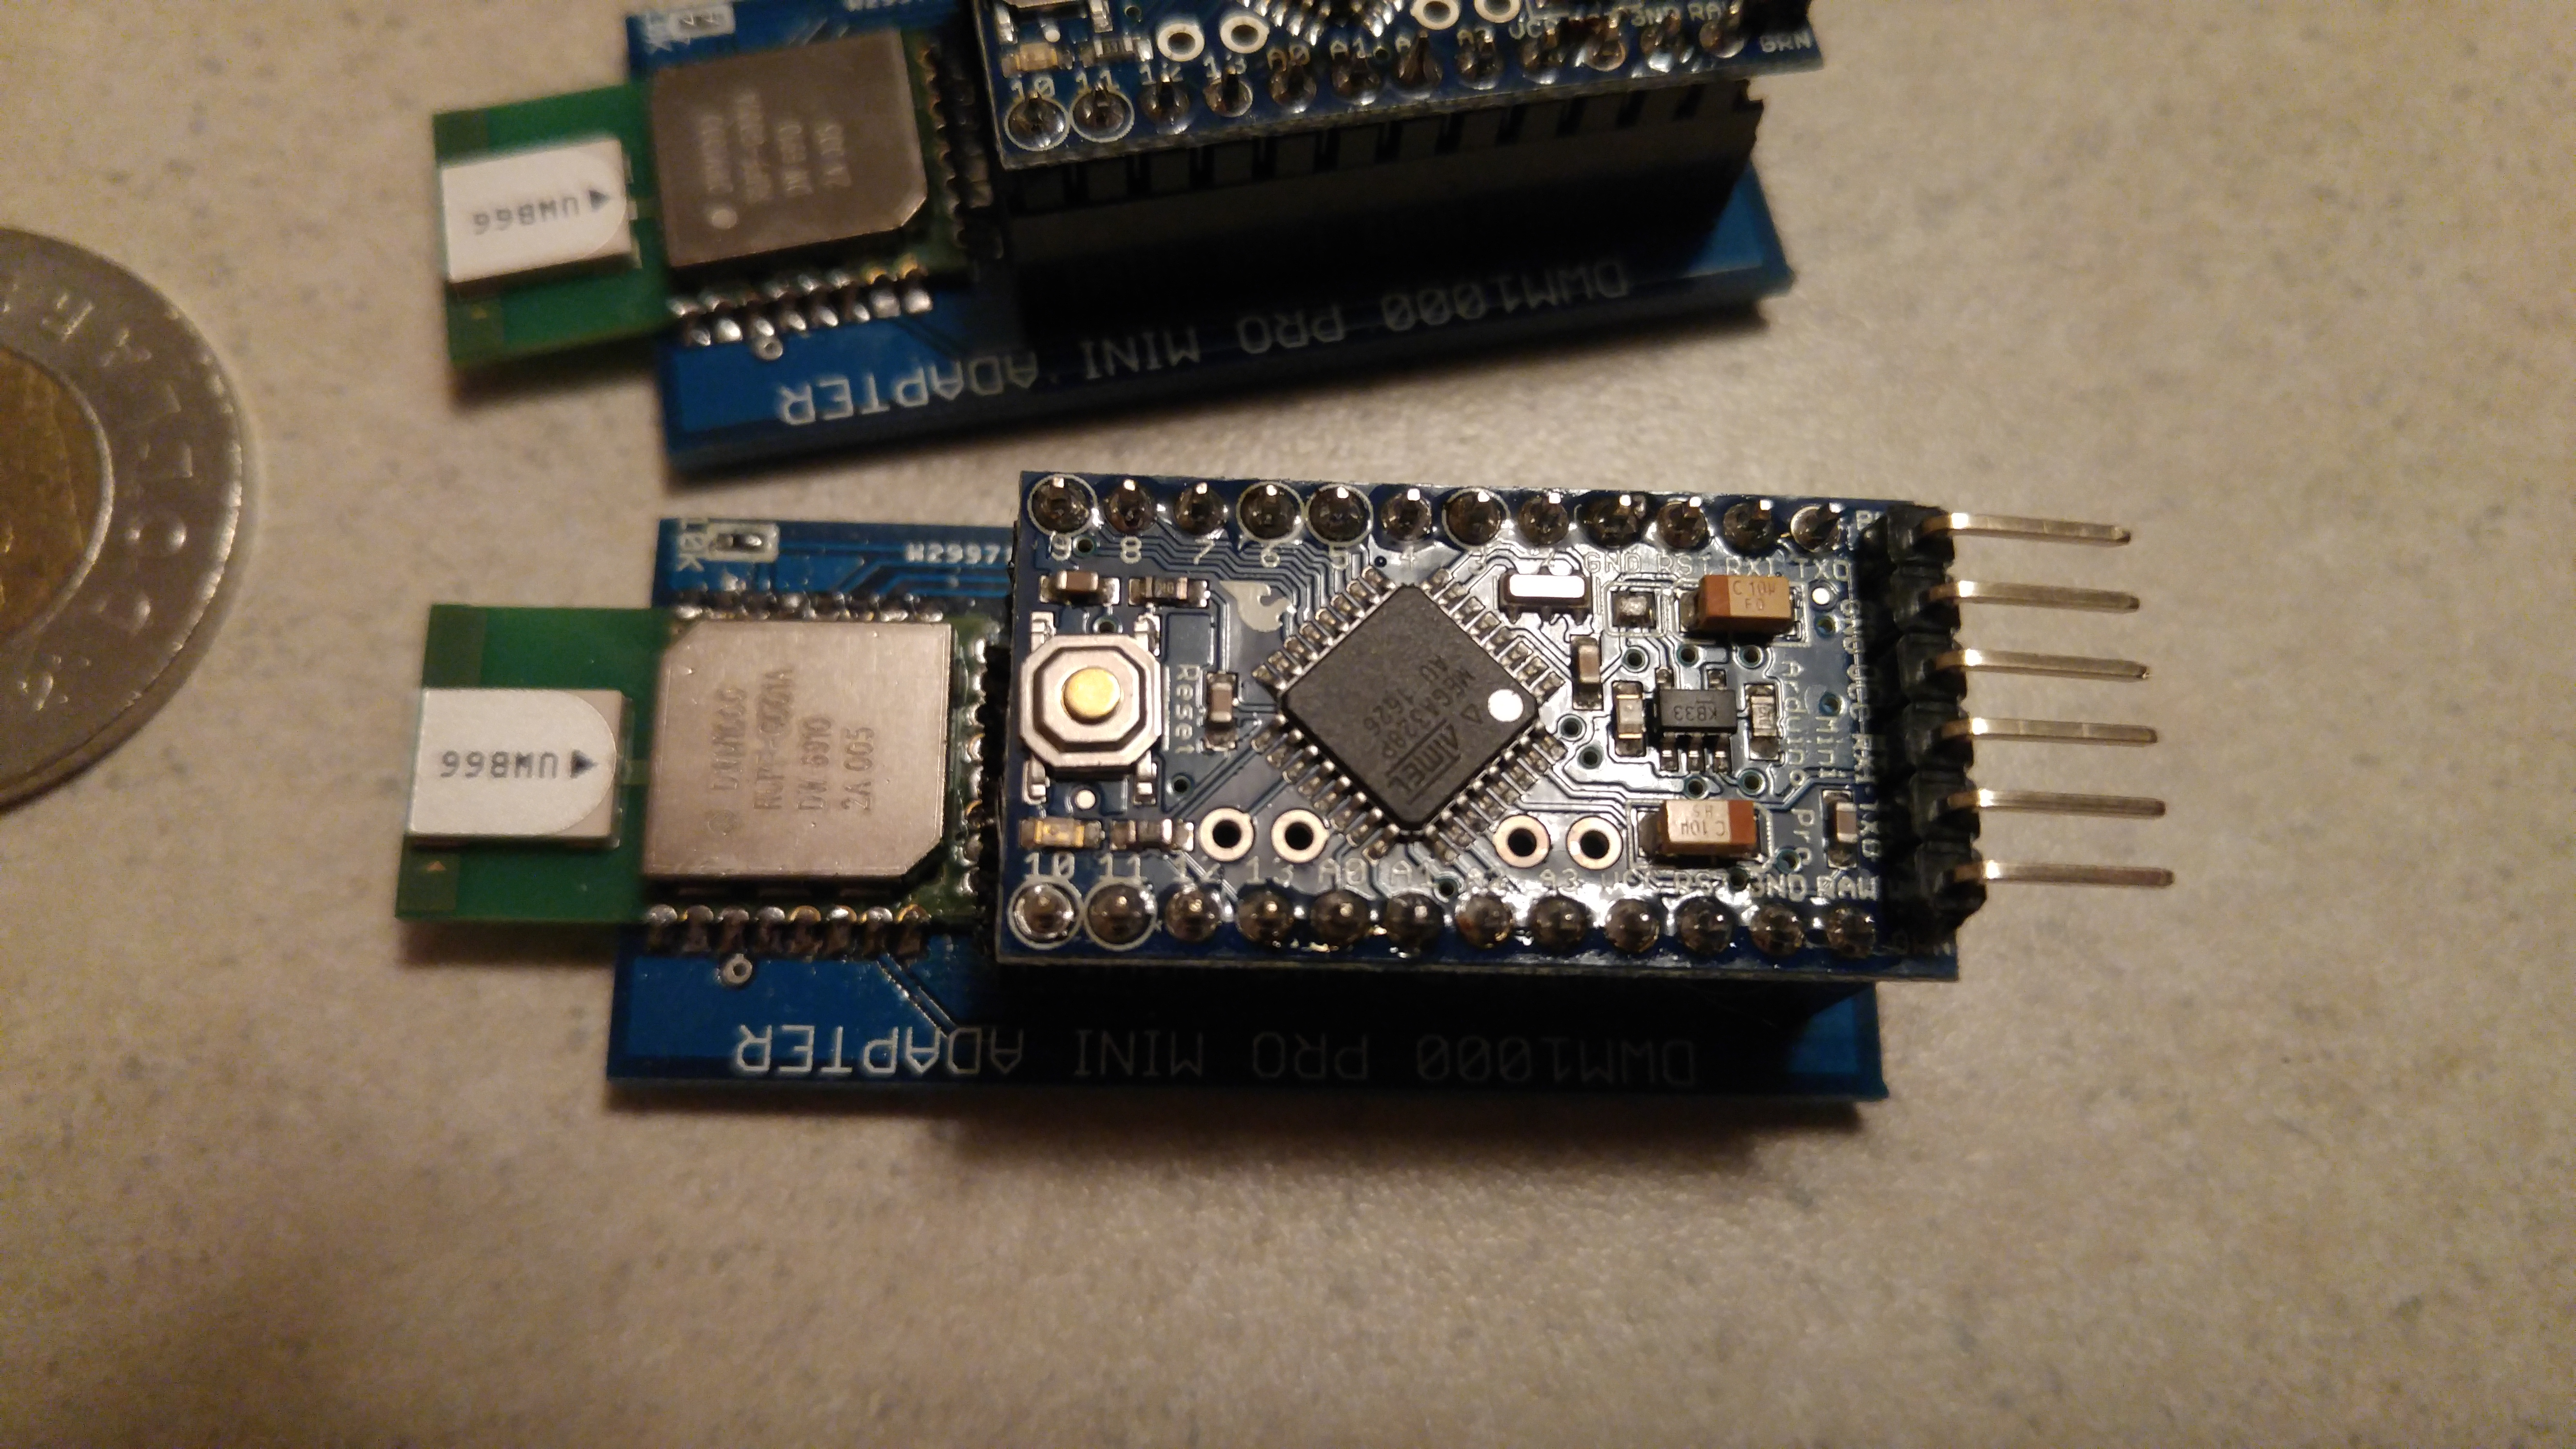
\includegraphics[width=\linewidth]{Figures/Tag.jpg}
	\decoRule
	\caption{A soldered tag.}
	\label{fig:Tag}
\end{figure}
The tags made for use with this project were required to be small enough to comfortably attach on a headset or cellphone. As the breadboards were too large, a custom PCB was designed.

Several designs were considered for the PCB connecting the Arduino and DWM1000. The most important factors were size and cost.

Several designs were considered at first:
\begin{itemize}
	\item The first idea considered was to place the Arduino and DWM on top of each other, resulting in the smallest possible size. However, the physical dimensions of the two components made this impossible. 
	\item Another possibility was to place each component on opposite sides of the PCB, but the Arduino's design demanded breakout headers to solder it into the board, which meant the PCB had to have holes drilled, which again meant that the physical dimensions of the two components interfered.
	\item Yet another idea was to make two PCBs. The Arduino would connect to a PCB above it, and that PCB would connect to a board above it with the DWM1000 soldered to it. Because it was layered, the pins connecting the layers could be arranged such that the Arduino and DWM1000 were essentially above each other, but without the locations of their pins interfering with each other. This design was abandoned because the breakout pins would add a large amount of vertical length, it was twice as expensive, and because it was much more complex to design.
	\item The final idea considered was to have the Arduino and DWM1000 just be placed next to each other on the same side of a PCB. This design was physically realizable, the least expensive, and though it was not as compact as would be ideal, it was still small enough to meet our requirements.
\end{itemize}

The last idea was chosen due to the its cheap cost, simplicity of design, and satisfactory size. 

As others who had used the DWM1000 recommended it \cite{LPSMini}, the PCB was designed so the antenna would not be on the PCB.

The PCB design was done in EAGLE and ordered from PCBWay. The PCB design can be seen in Figure~\ref{fig:PCB} and a soldered tag can be seen in Figure~\ref{fig:Tag}.

\section{Arduino Software}
The software to control the DWM1000 was written in C++ in Arduino IDE. The basic code to control the DWM1000 (handling memory address constants, communication with it via SPI, and a few high-level functions like send/receive) was available in Thomas ``thotro'' Trojer's open-source \code{arduino-dw1000} library. The library served as the foundation of the code used in this project to network the tags and anchors.

\subsection{Calculating a Delay}
\label{CalculatingADelay}
As part of the time-of-flight calculation, a timestamp is needed for when the ranging message was received and for when the reply was sent. The DWM1000 does not offer a way to automatically set the time upon transmission, but does offer the ability to set a time when a message will be transmitted in the future. If a delayed transmission is sent, the timestamp can be calculated ahead of time and then be embedded in the message.

Ideally, this delay is short. However, if the delay is too short, the Arduino will not be able to transmit the message data to the DWM1000 before the delayed timestamp is passed. This causes a silent error, and the DWM will not transmit anything. As well, the delay specified is not quite the delay at which the DWM1000 will begin transmitting, it is the delay that the DWM1000 will begin transmitting the data portion of the message. There is a ``premable'' sent before any transmission to allow the other devices in the network time to wake up and learn that a message is coming. Sending the preamble takes a relatively long time (approximately 1 microsecond per symbol in the preamble, which adds up to almost 2 ms for the preamble length chosen for this project). This was the most difficult to solve bug that was encountered in the design of the system.

The delay before a node can transmit is the sum of the:
\begin{itemize}
	\item Number of symbols in the preamble $\times$ 1\si{\micro\second} (2048 is the value used here, though the DWM offers different choices of preamble length, it is not exactly 1 \si{\micro\second} but it is very close)
	\item Time required to calculate and send the timestamp using SPI, about 1000\si{\micro\second} (empirically determined)
	\item Bytes of data to transmit $\times$ 4.5\si{\micro\second}, or 85 $\times$ number of devices in the network besides this one (empirically determined)
\end{itemize}

Adding in a fudge factor of about 200\si{\micro\second}, the delay we use in code for 6 devices is roughly 3500 \si{\micro\second}.

It is important to minimize this delay so as to increase the maximum frequency the system can update ranges at. The tradeoff of having a short preamble versus a long one is that a longer preamble takes time to send, but has a lower probability of being missed by the recipients. Tests indicated that the longest preamble, 2048 symbols, would be useful for in-door ranging due to the number of obstructions which would interfere with signals.  Shorter preambles resulted in missed messages a longer preamble could send without difficulty.

\section{Calibrating}
DWM1000s need to be calibrated to give correct distances due to the capacitance of the hardware connected to the chips, among other factors. Some of these factors are controlled for in software in the \code{arduino-dw1000} library. For a detailed overview of the possible errors and how to correct for them, the reader is advised to read the relevant sections in the DW1000 User Manual \cite{DW1000UserManual}.

The primary factor which could not be controlled for by the manufacturer, Decawave, was the antenna delay. The capacitance of the hardware the DWM1000 is hooked up to can cause nanosecond-level delays in transmission (in experiments, it was found that this could cause a meter of error or more incorrectly configured). This is a constant, and is determined empirically. The antenna delay constant for the tags is roughly the same. Good values were in the range of 16470-16500, and the antenna delay for the anchors is roughly the same and was found to be INSERT NUMBER HERE TODO.

Changing the antenna delay in the main code for easier calibration required changes to the \code{arduino-dw1000} library. A link to the code can be found in Appendix~\ref{ArduinoCode}.

\section{Results}
\label{RangefindingResults}
Results showed that the DWM1000 was close to as accurate as Decawave claimed (within 10cm). Of note, sometimes the reported ranges would glitch and be off by a meter or more. Table~\ref{tab:RangefindingAccuracy} shows the accuracy of the system. Though the accuracy of the rangefinding system was not a direct requirement of the project as a whole, the accuracy of the rangefinding system translates into accuracy of the position calculating system and thus the accuracy of the markers on the AR display.

\begin{table}
\caption{Accuracy of the rangefinding subsystem. Experiment performed with a tape measur and two tags lying on the ground. Antenna delay 16470.}
\label{tab:RangefindingAccuracy}
\centering
\begin{tabular}{c c c}
\toprule
\tabhead{Actual Distance (m)} & \tabhead{Mean Reported Distance (m)} & \tabhead{Standard Deviation (m)} \\
\midrule
0.5 & 0.62 & 0.045 \\
1 & 1.08 & 0.025 \\
2 & 2.24 & 0.03 \\
3 & 3.21 & 0.022 \\
4 & 4.22 & 0.104 \\
\bottomrule 
\end{tabular}
\end{table}

The operating frequency was close to the values predicted by the theory in Section~\ref{OperatingFrequencyAnalysis}. Predicted and actual values can be found in Table~\ref{tab:RangefindingFrequency}.

The max range between nodes was not determined due to space limitations but was at least 10m. The DWM1000 should get at least 60m if there are no obstructions \cite{DWM1000UserManual}.

\begin{table}
\caption{The frequencies of the rangefinding subsystem for various numbers of devices in the network. Experimented performed by placing an increasing number of devices in a network and calculating the duration between range reports from node 1 to node 2.}
\label{tab:RangefindingFrequency}
\centering
\begin{tabular}{c c c}
\toprule
\tabhead{Number of Devices} & \tabhead{Round Time (\si{\micro \second})} & \tabhead{Frequency (Hz)} \\
\midrule
2 & 37000 & 27 \\
3 & 58000 & 17.2 \\
4 & 86000 & 11.6 \\
5 & 93000 & 10.8 \\
6 & 156000 & 6.4 \\
7 & 170000 & 5.9 \\
\bottomrule
\end{tabular}
\end{table}

% Position Calculation


\chapter{Position Calculation} % Main chapter title

\label{PositionCalculation}

%----------------------------------------------------------------------------------------

This chapter covers the position calculation subsystem, which takes the ranges from the rangefinding subsystem and calculates their positions. It also covers how the subsystem is integrated into the augmented reality subsystem. The position subsystem is not a separate piece of hardware. Rather, it is just a very complex mathematical function. An example of possible positions calculated from range data is shown in Figure~\ref{fig:FrameOfReference}.

The topics covered in this chapter are:
\begin{enumerate}
	\item The infinite possible positions able to be calculated from a set of ranges.
	\item An example of calculating the positions of anchors with basic trigonometry in 2D.
	\item How this is extended to 3D.
	\item The protocol used by the Arduinos to communicate with the cell phones of the users and transfer the ranging data.
\end{enumerate}

\section{Frame of Reference}
\label{FrameOfReference}
\begin{figure}
	\centering
	\tikzstyle{vertex}=[circle, draw]
\begin{tikzpicture}[transform shape]
\node[vertex,label=below left:{(0, 0)}](a1) at (0, 0) {$ a_1 $};
\node[vertex,label=below left:{(3, 0)}](a2) at (3, 0) {$ a_2 $};
\node[vertex,label=below left:{(0, 4)}](a3) at (0, 4) {$ a_3 $};

\begin{scope}[every path/.style={-}, every node/.style={inner sep=1pt}]
       \draw (a1) -- node [anchor=north] {$3$} (a2);
       \draw (a2) -- node [anchor=south west] {$5$} (a3);
       \draw (a1) -- node [anchor=east] {$4$} (a3);
\end{scope} 

\node[vertex,label=above:{(-3, 3)}](a4) at (-3, 3) {$ a_1 $};
\node[vertex,label=below left:{(-6, 3)}](a5) at (-6, 3) {$ a_2 $};
\node[vertex,label=left:{(-3, -1)}](a6) at (-3, -1) {$ a_3 $};

\begin{scope}[every path/.style={-}, every node/.style={inner sep=1pt}]
       \draw (a4) -- node [anchor=south] {$3$} (a5);
       \draw (a5) -- node [anchor=north east] {$5$} (a6);
       \draw (a4) -- node [anchor=west] {$4$} (a6);
\end{scope} 
\end{tikzpicture}
	\decoRule
	\caption{Two example networks with different positions reporting the same ranges.}
	\label{fig:FrameOfReference}
\end{figure}

One of the most important aspects to understanding the position of an object in space is knowing what it is \emph{relative} to. If a point $p = (x, y, z) = (1, 2, 3)$, this is not useful unless it is known where, say, $(0, 0, 0)$ is and what directions the various axes point in.

The rangefinding subsystem determines the ranges between various devices. With these ranges, trigonometry can be used to determine positions in 3D space. However, it is impossible to place the positions in such a way that they correspond to the real world with only the range information. There are many different possible sets of positions which will result in the same rangefinding data. Figure~\ref{fig:FrameOfReference} shows two possible sets of positions that will result in the rangefinding system reporting the same ranges.

In order to cut down on the infinite possible solutions to finding positions given only range data, this subsystem must arbitrarily create its own system of coordinates. The positions calculated by this subsystem must be further transformed so as to correspond to the real world. This transformation is not covered in this chapter, and instead is dealt with in Section~\ref{Calibration}.

\section{Starting in 2D}
\label{HighLevelExample}

\begin{figure}
	\centering
	\tikzstyle{vertex}=[circle, draw]
\begin{tikzpicture}[transform shape]
\node[vertex](a0) at (0, 0) {$ a_0 $};
\node[vertex](a1) at (6, 0) {$ a_1 $};
\node[vertex](a2) at (1.5, 4.3) {$ a_2 $};


\begin{scope}[every path/.style={-}, every node/.style={inner sep=1pt}]
       \draw (a0) -- node[align=center, anchor=north] {$d_{01}$} (a1);
       \draw (a0) -- node[align=center, anchor=south east] {$d_{02}$} (a2);
       \draw (a1) -- node[align=center, anchor=south west] {$d_{12}$} (a2);
\end{scope} 
\end{tikzpicture}
	\decoRule
	\caption{A network with 3 anchors $a_i$ and the reported distances between them.}
	\label{fig:PositionCalculationNetwork}
\end{figure}

As 3D position calculation is much more complex, position calculation is done in 2D will be explained first. The distances between three anchors, $a_{0}$, $ a_{1}$  and $a_{2}$ are obtained first. The distance between anchor $i$ and anchor $j$ is $d_{ij}$. This network is shown in Figure~\ref{fig:PositionCalculationNetwork}.

In order to assign positions in 2D space to the anchors that keep them the same ranges from each other, $a_{0}$ is set arbitrarily to be at the origin. Next, $a_{1}$ is arbitrarily decided to be on the x-axis, which puts it at the position $(0, d_{01})$. With these two positions, the angle $\Theta$ between the x-axis and the vector from $a_0$ to $a_2$ can be calculated with the cosine law:

\[ \Theta = \cos ^{-1}\Big(\frac{d_{01}^2 + d_{02}^2 - d_{12}^2 }{2 d_{01} d_{02}}\Big)\]

With $\Theta$, we can calculate x and y coordinates of $a_2$:

\[ x = cos(\Theta) d_{12} \]
\[ y = sin(\Theta) d_{12} \]

\section{3D Position Calculation}
Extending the subsystem to three dimensions starts the same way as in two dimensions, though four anchors are required to get a reliable position in 3D. We have our four anchors: $a_{0}$, $a_{1}$ , $a_{2}$ and $a_{3}$. 

To begin, the same steps are followed as detailed in Section~\ref{HighLevelExample}, but the z-coordinate of every point is set to 0. That is, the origin is arbitrarily determined to be the position of $a_{0}$. $a_{1}$ is arbitrarily determined to be on the x-axis and placed at $(0, d_{01}, 0)$, where $d_{01}$ is the distance between $a_{0}$ and $a_{1}$. The cosine law is then used to determine the position of $a_{2}$.

The calculation of the position of the fourth anchor comes last. As the other three anchors have been declared as being on the xy-axis, the fourth anchor must contain a z-component.

To begin with, we calculate the $(x, y)$ position of the fourth anchor as if it were on the xy-plane - though only temporarily.

\[ \Theta = \cos ^{ - 1}\Big(\frac{d_{01}^2 + d_{03}^2 - d_{13}^2 }{2 d_{01} d_{03}}\Big)\]

\[ x_{temp} = cos(\Theta) d_{13} \]
\[ y_{temp} = sin(\Theta) d_{13} \]
\[ z_{temp} = 0 \]

This temporary point is the correct distance from all the anchors except $a_3$. In order to determine a position that is the correct distance away from $a_2$ but still the same distance away from $a_0$ and $a_1$, the temporary point is rotated around the x-axis. Because the first two anchors are on the x-axis, this keeps their distance to $a_3$ constant.

This rotation forms a circle around the x-axis of a radius equal to $y_{temp}$. We will rotate our temporary point to a position where its distance from $a_2$ is equal to $d_{23}$.

We calculate the distance between the x value of the temporary point and the x value of anchor 2, we denote this value $\Delta x$.

\[ \Delta x = x_{temp} - x_{2} \]

Now that we have $\Delta x$ we can now calculate the position of our fourth anchor using trigonometry:

\[\Theta = \cos ^{ - 1}\Big(\frac {\Delta x^2 - d_{23}^2 + y_{2}^2 + y_{temp}^2}{2 y_{2} y_{temp}}\Big)\]

A proof for this equation can be found in Appendix~\ref{PositionCalculationProof}.

There are two possible values for $\Theta$, positive or negative. The decision affects whether our anchor has a positive or negative z-component. The positive z-component is chosen arbitrarily; the cell phone calibration process can flip the z-component later.

\[ x_{3} = x_{temp} \]
\[ y_{3} = cos(\Theta) y_{temp} \]
\[ z_{3} = sin(\Theta) y_{temp} \]

\section{Integrating Rangefinding and Position Calculation}
The position calculation code runs on the cellphone. In order to calculate positions, ranges must be transferred to the cellphone from the Arduino Pro Mini. 

The Arduino's processor can communicate serially via UART TTL. Most cellphones do not have the ability to communicate serially, but Future Technology Devices International (FTDI) manufactures a USB cable that interfaces between the serial output of the Arduino and the micro USB port of a cellphone. With this cable connecting an Arduino and a cellphone, the cellphone can provide power to the Arduino and send and receive data to it.

The project uses the Android \code{D2xx} library, provided by FTDI, to communicate with the Arduino while running an Android app. It allows the easy sending and receiving of bytes. 

\section{Protocol}
There are a number of design considerations when dealing with the communications between the cellphone and the Arduino:
\begin{enumerate}
	\item The stream of data may begin in the middle of a message, as the buffer storing the serial data sent from the Arduino has only a limited capacity. If a cellphone were connected to an anchor that had already been running for some time, it is quite likely that the buffer would have overflowed. So, the protocol must include a way to determine the start of a message.
	\item The protocol should be human readable for easy debugging.
\end{enumerate}

With this in mind, a simple protocol was developed. Lines of text, delineated by newline characters, are sent. If the Arduino is reporting the range between two devices, it sends a line with the format:

\begin{center}
\code{!range <from ID> <to ID> <range in meters>}
\end{center}

If the Arduino is informing the cellphone of its id, it sends a line with the format:

\begin{center}
\code{!id <tag's ID>}
\end{center}


If the cellphone reads a line which does not start with `!', the line is assumed to either have started in the middle of a ranging information line, or else debug data has been sent. Either way, the line is discarded and the system waits to read a new line.

An example of the output from the Arduino is:

\code{\\
DW1000 initialized ... \\
Committed configuration ... \\
New device found. ID: 1 \\
Transmission received from tag 1 with transmission count 1 \\
!range 1 2 0.00 \\
Transmission received from tag 1 with transmission count 3 \\
!range 2 1 3.26 \\
!range 1 2 91659.28 \\
Transmission received from tag 1 with transmission count 5 \\
!range 2 1 3.48 \\
!range 1 2 3.38 \\
Transmission received from tag 1 with transmission count 7 \\
!range 2 1 3.37 \\
!range 1 2 3.42 \\
}

Note the briefly extremely large range while the timestamps settle.

Parsing is done on the cellphone with the \code{java.util.Scanner} class. The parsing code can be found in \code{TagParser.java} in the AR Code. See Appendix~\ref{SourceCode}.

\section{Summary}
This chapter covered the position calculation subsystem.

The issues with the infinite possible positions that can be calculated from a set of ranges between nodes were raised. Ultimately the positions calculated by this system must be calibrated by the cell phone to correspond to real world positions.

The math behind calculating positions in 3D given distances between nodes was discussed. The key to solving for the position of the fourth anchor is through making a circle around the x-axis and finding out where on the circle to place the fourth anchor so that the distance from it to anchor 3 matches.

Finally, the specifics of how the cellphones and Arduinos are interfaced were discussed. The Arduino, which holds the range information, is connected to the cell phone via a USB cable which translates the serial output of the Arduino into a stream of bytes for the cell phone to read and parse. Messages can be corrupted on occasion or be received halfway through, so each important message starts with a `!' character.
% Augmented Reality

\chapter{Augmented Reality} % Main chapter title

\label{AugmentedReality}

%----------------------------------------------------------------------------------------

This chapter covers the AR portion of the project. The AR subsystem takes the positions from the position calculation subsystem and renders them on the screen of a cellphone using OpenGL. If they cannot be directly rendered, an arrow is drawn on the edge of the screen to show which way the object is from the user. An example of this can be found in Figure~\ref{dfis} (DO THIS FIGURE).

The code for the AR subsystem can be found at (PROVIDE LINK HERE).

This chapter covers the following topics:
\begin{enumerate}
	\item A brief overview of the math used later in this section, including homogenous coordinates and transformation matrices.
	\item A description of OpenGL and the basics of how it is used. 
	\item How objects and text can accurately be drawn on the screen overlaid on a camera image.
	\item How the coordinate system of the position calculation system can be transformed into real world coordinates through the cell phone's sensors.
	\item Examples of the accuracy of the subsystem.
\end{enumerate}

\section{3D Math Overview}
This section covers the basics of using matrices to render 3D scenes. A full treatment of the subject is beyond the scope of this report, though other resources on the subject exist (PUT CITATION HERE). The reader is assumed to be familiar with some linear algebra, including the multiplication of matrices. 

\subsection{Transformation Matrices}
\begin{figure}
	\centering
	\begin{minipage}{.33\textwidth}
		\centering
		\includegraphics[width=\linewidth]{Figures/Translation.png}
	\end{minipage}
	\begin{minipage}{.33\textwidth}
		\centering
		\includegraphics[width=\linewidth]{Figures/Rotation.png}
	\end{minipage}
	\begin{minipage}{.33\textwidth}
		\centering
		\includegraphics[width=\linewidth]{Figures/Scaling.png}
	\end{minipage}
	\decoRule
	\caption{Translation, rotation, and scaling of vectors are all possible with matrices \cite{OpenGLMatrices}.}
	\label{fig:Transformations}
\end{figure}

\textbf{Transformation matrices} are matrices which can describe transformations in space such as translation, rotation, and scaling. They are regularly used in computer graphics. 

Figure~\ref{fig:Transformations} shows some of the transformations that can be applied to vertices with matrices.

Transform matrices can be composed with multiplication. For example, one could describe the translation of a point with a translation matrix, then multiply the matrix by a rotation matrix to create a new matrix which, when multiplied by a vector, cause that vector to be rotated and then translated.

Order matters when composing transformation matrices. The matrix $\mathbf{T} \mathbf{R}$ is not the same as $\mathbf{R} \mathbf{T}$.

Normally, the transformation of a vector $v$ to a new vector $v'$ with a transformation matrix $\mathbf{M}$ is written as:

\[ v' = \mathbf{M} v \]

Or, with two transformation matrices $\mathbf{M_1}$ and $\mathbf{M_2}$ composed:

\[ v' = \mathbf{M_2} \mathbf{M_1} v \]

When written like this, the transformation matrix $\mathbf{M_1}$ can be viewed as applying to the vector first, and then the new transformed will be further transformed by $\mathbf{M_2}$.

In this report, points and vectors will be used interchangeably. When a matrix is said to multiply a point $p = (x, y, z)$, it should be considered as multiplying a vector $v = \begin{bmatrix}x & y & z\end{bmatrix}^T $. 

The definitions of matrices which scale, translate, and rotate are mostly beyond the scope of this report. OpenGL provides utility functions to create them, so the exact definitions are unnecessary.

\subsection{Homogenous Coordinates}
For a given 3$\times$3 matrix $M$ and an arbitrary point in 3D space $p = (x, y, z)$, there is no $\mathbf{M}$ such that will multiplying it by any $p$ will cause $p$ to be translated by a specified number of units. There is, however, a way to do it with a homogenous point and a 4x4 matrix. This is one of the reasons homogenous coordinates are used in OpenGL.

\textbf{Homogenous coordinates} are coordinates in space which contain an extra element $w$ which acts as a scaling factor on the three elements. A 3D homogenous coordinate $p_h$ could be written as:

\[ p_h = (x_h, y_h, z_h, w) \]

This relates to a regular point in 3D space:

\[ (x, y, z) = (\frac{x_h}{w}, \frac{y_h}{w}, \frac{z_h}{w}) \] 

For example, the homogenous point $(1, 1, 1, 1)$ maps to the regular 3D point $(1, 1, 1)$. The homogenous point $(2, 2, 2, 2)$ does as well.

A translation matrix $T$ that moves a point $p$  by $(T_x, T_y, T_z)$ units, is:

\[
\mathbf{T} = \begin{bmatrix}
1 & 0 & 0 & T_x \\
0 & 1 & 0 & T_y \\
0 & 0 & 1 & T_z \\
0 & 0 & 0 & 1
\end{bmatrix}
\]

To prove this, we'll multiply out a homogenous point $p_h = (x_h, y_h, z_h, w)$ by $\mathbf{T}$ and show that, when converted to a regular 3D point, it equals $(\frac{x}{w} + T_x, \frac{y}{w} + T_y, \frac{z}{w} + T_z)$.

\[ p_{h}\prime = \mathbf{T} p_h \]

\[
  p_{h}\prime = \begin{bmatrix}
1 & 0 & 0 & T_x \\
0 & 1 & 0 & T_y \\
0 & 0 & 1 & T_z \\
0 & 0 & 0 & 1
\end{bmatrix} 
\begin{bmatrix}
x_h \\ y_h \\ z_h \\ w 
\end{bmatrix}
\]

\[
 p_{h}\prime = \begin{bmatrix}
 x_h + w T_x \\
 y_h + w T_y \\
 z_h + w T_z \\
 w
 \end{bmatrix}
 \]
 
 Now, if we convert $p_{h}\prime$ to a regular 3D point $p$, we get:
 
 \[ p = (\frac{x_h}{w} + \frac{w T_x}{w},  \frac{y_h}{w} + \frac{w T_y}{w}, \frac{z_h}{w} + \frac{w T_z}{w}) \]
 \[ p = (x/w + T_x, y/w + T_y, z/w + T_z) \]
 
 which is the translation of $p$ by $(T_x, T_y, T_z)$ units.
 
 \section{OpenGL}
\textbf{OpenGL} is an API used to render 2D and 3D graphics. For the project, OpenGL was used to render position markers in 3D space overtop what the cell phone's camera sees.

OpenGL works by taking in collections of points making up a 3D model of an object and then applying various matrix transforms to the points, translating and rotating them. Afterwards, it projects them onto a 2D plane and renders them. A full treatment of how OpenGL works is beyond the scope of this report, but (INSERT CITATION HERE FOR OPENGL BOOK).

The three main matrices that OpenGL uses to render a 3D scene are called the \textbf{projection matrix}, \textbf{view matrix}, and \textbf{model matrix}. This project uses several novel techniques which use and manipulate the matrices that OpenGL uses to render a 3D scene. This report will only cover them briefly, though other resources explore them more fully \cite{CodingLabs}.

\section{The Model Matrix}
\begin{figure}
	\centering
	\tikzstyle{vertex}=[circle, draw]
\begin{tikzpicture}[transform shape]
\draw[->,ultra thick] (0,0, 0)--(3,0, 0) node[right]{$x$};
\draw[->,ultra thick] (0,0, 0)--(0,3, 0) node[above]{$y$};
\draw[->,ultra thick] (0,0, 0)--(0,0, 5) node[below left]{$z$};

\node[vertex,inner sep=2pt,minimum size=1pt,label=left:{$(-1, -1, 0)$}](v1) at (-1, -1, 0) {};
\node[vertex,inner sep=2pt,minimum size=1pt,label=below right:{$(1, -1, 0)$}](v2) at (1, -1, 0) {};
\node[vertex,inner sep=2pt,minimum size=1pt,label=above right:{$(1, 1, 0)$}](v3) at (1, 1, 0) {};
\node[vertex,inner sep=2pt,minimum size=1pt,label=above left:{$(-1, 1, 0)$}](v4) at (-1,1, 0) {};

\begin{scope}[every path/.style={-}, every node/.style={inner sep=0pt}]
       \draw (v1) -- node [anchor=south east] {} (v2);
       \draw (v2) -- node [anchor=south west] {} (v3);
       \draw (v3) -- node [anchor=north] {} (v4);
       \draw (v4) -- node [anchor=north] {} (v1);
\end{scope} 
\end{tikzpicture}
	\decoRule
	\caption{An example 3D model of a square in model coordinates.}
	\label{fig:ModelExample}
\end{figure}
\begin{figure}
	\centering
	\tikzstyle{vertex}=[circle, draw]
\begin{tikzpicture}[transform shape={scale=0.4}]
\draw[->,ultra thick] (0,0, 0)--(5,0, 0) node[right]{$x$};
\draw[->,ultra thick] (0,0, 0)--(0,5, 0) node[above]{$y$};
\draw[->,ultra thick] (0,0, 0)--(0,0, 5) node[below left]{$z$};

\node[vertex,inner sep=2pt,minimum size=1pt,label=below:{$(-6, -1, 0)$}](v1) at (-6, -1, 0) {};
\node[vertex,inner sep=2pt,minimum size=1pt,label=below right:{$(-4, -1, 0)$}](v2) at (-4, -1, 0) {};
\node[vertex,inner sep=2pt,minimum size=1pt,label=above right:{$(-4, 1, 0)$}](v3) at (-4, 1, 0) {};
\node[vertex,inner sep=2pt,minimum size=1pt,label=above:{$(-6, 1, 0)$}](v4) at (-6,1, 0) {};

\node[vertex,inner sep=2pt,minimum size=1pt,label=left:{$(4, -1, 0)$}](v5) at (4, -1, 0) {};
\node[vertex,inner sep=2pt,minimum size=1pt,label=below right:{$(6, -1, 0)$}](v6) at (6, -1, 0) {};
\node[vertex,inner sep=2pt,minimum size=1pt,label=above right:{$(6, 1, 0)$}](v7) at (6, 1, 0) {};
\node[vertex,inner sep=2pt,minimum size=1pt,label=above left:{$(4, 1, 0)$}](v8) at (4,1, 0) {};

\begin{scope}[every path/.style={-}, every node/.style={inner sep=0pt}]
       \draw (v1) -- node [anchor=south east] {} (v2);
       \draw (v2) -- node [anchor=south west] {} (v3);
       \draw (v3) -- node [anchor=north] {} (v4);
       \draw (v4) -- node [anchor=north] {} (v1);
       
       \draw (v5) -- node [anchor=south east] {} (v6);
       \draw (v6) -- node [anchor=south west] {} (v7);
       \draw (v7) -- node [anchor=north] {} (v8);
       \draw (v8) -- node [anchor=north] {} (v5);
\end{scope} 
\end{tikzpicture}
	\decoRule
	\caption{A 3D scene with two squares, the centers of which are placed at $(5, 0, 0)$ and $(-5, 0, 0)$ in world coordinates by transforming the vertices of Figure~\ref{fig:ModelExample} with two model matrices.}
	\label{fig:ModelMatrixExample}
\end{figure}

The model matrix exists to take \textbf{model space}, in which the coordinates of a 3D model are relative to the center of the model, and transform it into \textbf{world space}, in which coordinates are relative to the center of the ``world''. Most of the code in this project considers the locations of objects in world space. For example, the position subsystem might say that a tag is at $(5, 5, 1)$. This coordinate is considered to be in world space, though it should be noted that this is not the same as \emph{real} world coordinates - a further transform is required to match up the positions given by the position calculation subsystem with the real world as shown by a camera.

Figure~\ref{fig:ModelExample} shows an example of a square in model space. The square's 3D model has its vertices placed at $(-1, -1, 0)$, $(1, -1, 0)$, $(1, 1, 0)$, and $(-1, 1, 0)$. An example of creating a 3D scene with two squares at $(5, 0, 0)$ and $(-5, 0, 0)$ in world coordinates can be seen in Figure~\ref{fig:ModelMatrixExample}. A model matrix is created for each of the squares. The first model matrix encodes a translation $(-5, 0, 0)$ units and the second model matrix encodes a translation of $(5, 0, 0)$ units. To get the vertices of the first square in world coordinates, the first model matrix is applied to the square's vertices. The same is done for the second square and model matrix. 

That is, for the model matrix $\mathbf{M}$ and each vertex $v$ of the square, the vertex $v$ is transformed into world coordinates vertex $v'$ by the formula:

\[v' = \mathbf{M}v \]

\section{The View Matrix}
\begin{figure}
	\centering
	\includegraphics[width=\linewidth]{Figures/WorldToView.png}
	\decoRule
	\caption{A figure showing an object in world coordinates and an object in camera coordinates \cite{CodingLabs}.}
	\label{fig:WorldToView}
\end{figure}

In a 3D scene, a position is declared from which the scene is viewed. The view matrix exists to transform world coordinates to \textbf{view space}, in which coordinates are relative to the position from which the scene is viewed. It as if an imaginary camera has been placed in the scene. Figure~\ref{fig:WorldToView} shows an example of this.

The view matrix is typically just a simple translation of all the vertices (if a camera is placed at $(5, 5, 5)$, then all the vertices will be translated by $(-5, -5, -5)$), and then a rotation based in which direction the camera is looking at. 

For the rest of this project, the imaginary camera is assumed to be located at (0, 0, 0), making the view matrix a simple rotation matrix. The positions of markers and objects are calculated relative to the position of the tag connected to the cellphone.

\section{The Projection Matrix}

\begin{figure}
	\centering
	\includegraphics[width=\linewidth]{Figures/ProjectionMatrix.png}
	\decoRule
	\caption{The transformation from view space to projection space \cite{CodingLabs}.}
	\label{fig:ProjectionMatrix}
\end{figure}

\begin{figure}
	\centering
	\includegraphics{Figures/ProjectionMatrix2.png}
	\decoRule
	\caption{A teapot in projection space \cite{CodingLabs}.}
	\label{fig:ProjectionMatrix2}
\end{figure}

In one of the last steps in rendering a 3D scene in OpenGL, the scene must be projected onto a plane so it can be displayed on a monitor. The projection matrix is involved in this process. View space is transformed into \textbf{projection space}, in which coordinates are transformed into \textbf{normalized device coordinates} (NDCs). Vertices which fall within the field of view will be contained within a cube with corners $(-1, -1, -1)$ and $(1, 1, 1)$ and are drawn. Vertices outside this box are culled. 

There are different types of projection matrices. For the purposes of this projection, only the \textbf{perspective projection matrix} is considered. This projection takes into account that objects which are further away from the camera should appear smaller. Figure~\ref{fig:ProjectionMatrix} and Figure~\ref{fig:ProjectionMatrix2} show the transform from view space to projection space via a perspective projection matrix.

To actually render the image in 2D, the NDCs are converted to the coordinates of pixels as determined by the size of the surface being rendered to. The $z$ coordinates handle depth, which allows OpenGL to determine whether a shape is on top of another during the rendering process.

\section{Camera Perspective and OpenGL Perspective}
\begin{figure}
	\centering
	\includegraphics[width=\linewidth]{Figures/CameraLens.png}
	\decoRule
	\caption{A diagram depicting the field of view of a camera \cite{MartyBugs}.}
	\label{fig:CameraLens}
\end{figure}
In order to accurately display the locations of the devices, it is important that the 3D scene rendered by OpenGL match up with the real world as shown by the cellphone's camera. Figure~\ref{fig:CameraLens} shows how a camera can only see see a limited part of the world, as dictated by its field of view.

As previously shown in Figure~\ref{ProjectionMatrix}, the projection matrix has a field of view which can be changed. The field of view for the OpenGL perspective matrix needs to be set on a per-cellphone basis to match that of the cellphone's camera for the project to display locations accurately.

(TODO FINISH THIS UP LATER WITH MORE DETAIL IF TIME PERMITS.)

\section{Cellphone Rotation}
\begin{figure}
	\centering
	\includegraphics[width=6cm]{Figures/AxisDevice.png}
	\decoRule
	\caption{The coordinate system used by the Android Sensor API \cite{AndroidSensorDocsOverview} and by AR subsystem, assuming the phone's top points towards geomagnetic North and the screen points toward the sky. For the purposes of rotation, X points approximately East, Y to geomagnetic North, and Z towards the sky \cite{AndroidSensorDocs}.}
	\label{fig:CameraLens}
\end{figure}

In order to display the positions of markers on the screen correctly, the direction the camera is facing must be known. The cellphone can determine this by requesting the phone's rotation from Android's Sensor API. Android does not specify \emph{how} the rotation of the phone is determined, but in practice uses a subset of the magnetometer, accelerometer, and gyroscope (if the phone contains these sensors; Android does not force phone manufacturers to include any of these sensors). 

For example, if the phone has a magnetometer and an accelerometer, by determining the direction of magnetic north and the direction of the force of the gravity on the phone, the direction of the phone's rotation can be determined \cite{AndroidSensorDocs}.

The cellphone has its own coordinate system which must be taken into account. To deal with the coordinate system differences, the Android Sensor API includes a method to remap the coordinate system of the rotation it reports. The coordinate system used by the project for its real world coordinates was chosen to match the coordinate system of the Android Sensor API, which can be seen in Figure~\ref{fig:RotationCoordinateSystem}.

The rotation value returned by the Android OS was found to be quite accurate in tests so long as the device was not in motion. If the device was in freefall or moving, it became more difficult for the Android OS to determine the direction of gravity, which in turn made the calculated rotation values inaccurate.

The Android Sensor API can directly return a rotation matrix. However, the way it is stored in memory is not quite the same as how OpenGL stores matrices, so the matrix must be transposed before being used in OpenGL.

The rotation matrix returned is used in the project to create the view matrix by taking a ``lookAt'' vector equal to $(0, 0, -1)$ (which represents that the camera, when at `rest' on a table looks down the z axis) and ``up'' vector equal to $(0, 1, 0)$ (arbitrarily stating that the `up' direction of the cellphone screen points north) and rotating each by the rotation matrix returned by the phone. The new vectors produced are then used in the OpenGL utility function \code{setLookAtM} which creates a view matrix based on an up vector and the point at which the camera should be looking at.

The rotation matrix could have been used directly as the view matrix without going through these steps. However, for later processing it is necessary to have the lookAt and up vectors rotated. 

Thus, if we ignore the transformation required to correct for the arbitrary coordinate system of the position calculation subsystem, the view matrix, $\mathbf{V}$, every frame is to set it equal to the rotation matrix the Android OS last returned, $\mathbf{R_{cur}}$:

\[
	\mathbf{V} = \mathbf{R_{cur}}
\]

\section{Calibration}
As noted in Section~\ref{FrameOfReference}, the positions calculated by the position calculation subsystem have an arbitrary coordinate system where the XY plane is formed by the positions of the three anchors with the lowest ID and the Z axis is determined by the fourth anchor. In order to display positions obtained from this subsystem accurately on top of the images captured by the cellphone's camera, there is a necessary calibration step on system startup to create a transformation matrix which can convert coordinates into the cell phone's coordinate system. The user determines the transformation needed to convert to the coordinate system used by the cellphone by rotating and positioning the phone until it displays the position of a device correctly, at which point the system knows the transformation needed.

The steps a user follows to calibrate the system are:
\begin{enumerate}
	\item The user taps the phone's screen to enter calibration mode.
	\item The system creates a new view matrix every frame which will cause the screen to display the position of an arbitrary device in the network in the middle of the screen.
	\item The user then points the phone directly at the tag being displayed and rotates the phone until the position of a second tag matches its location on the screen.
	\item The user then taps the screen to end calibration mode. The system stores the view matrix at this time, $\mathbf{V}_{end}$, as well as the raw rotation matrix at the time, $\mathbf{R}_{end}$.
	\item If the locations of other tags are incorrect due the z-axis being flipped (the z axis of the position calculation subsystem flips based on the elevation of the anchor with the highest ID), the user taps the phone's screen twice to correct it. The system stores this in a boolean and, when calculating the positions of other devices relative to the user's location, knows whether to flip the z component.
\end{enumerate}

(TODO INSERT PICTURE HERE)

Each frame, to correctly position the objects, the calibration matrix should be changed only by the rotation of the device from its rotation at the end of the calibration. Before, each frame the view matrix was set equal to the current raw rotation matrix, $\mathbf{R}_{cur}$. Now, the view matrix must multiplied by a matrix to correct for the coordinate transform. Intuitively, this calibration matrix should reverse the effects of the rotation at the end of the calibration mode and multiply by the view matrix at the time. A rotation can be reversed by inverting the matrix. Thus, the new calibrated view matrix used every frame, $\mathbf{V}_{cal}$, is:

\[ 
	\mathbf{V}_{cal} = \mathbf{V}_{end} \mathbf{R}^{-1}_{end} \mathbf{R}_{cur}
\]

\section{Billboarding}
\begin{figure}
	\centering
	\includegraphics[width=8cm]{Figures/Billboarding.png}
	\decoRule
	\caption{Billboarding used to make objects O1, O2, and O3 face the camera \cite{Lighthouse3D}.}
	\label{fig:Billboarding}
\end{figure}
So far, this chapter has discussed how a collection of vertices can be transformed, and more specifically how the positions of other devices can be correctly placed. This would be sufficient if the system had to render a cube at the position of the object in question. Aesthetically, rendering a cube would leave a lot to be desired. This section covers a method to draw a 2D image at a 3D location.

\textbf{Billboarding} is a technique to make an object face the screen no matter where it is situated. It is used, for example, in some 3D games to render trees as 2D images to lower the number of vertices that need to be processed in a scene. Figure~\ref{fig:Billboarding} shows the end result of using billboarding for 2D objects.

There are many ways to do billboarding, depending on whether you want to only have the object rotate on a specific axis \cite{Lighthouse3D}. For this project, it was determined that the best way to represent an object's position on the screen was to have a rotating circular 2D image as a marker. The exact graphic used was chosen for aesthetic reasons.

To have this 2D image always face the screen, it must be able to rotate on all three axes. The technique to accomplish this rotation is to multiply the model matrix before it is translated by the inverse of the portion of the view matrix corresponding to rotation. That is, given a model matrix $\textbf{M}$, making it rotate to always face the camera is accomplished by creating a new billboarding model matrix $\textbf{M}_b$:

\[ \textbf{M}_b = \textbf{M} \textbf{V}^{-1} \]

Intuitively, when a model's vertices are multiplied by the view matrix, they are rotated about depending on the angle the camera is facing. If we reverse this rotation effect but not the translation part, the model will always face the camera.

As the camera is always situated at $(0, 0, 0)$ in this project, multiplying the model matrix of the textured square by the inverted view matrix will produce a billboarding effect. If we first rotate the square about the Z-axis (assuming the square's vertices are on the XY plane), it will produce the rotating effect on the final image.

\section{Marking the Positions of Objects Off-Screen}
One of the advantages of AR is the ability to put more information on the screen than can be seen with the human eye. As part of the goal of the project to increase the user's awareness of the locations of objects, the system informs the user of where an object is relative to them when the object is not within the viewing area of the camera.

First, the system needs to determine whether or not the objection is within the viewing area. This is done by multiplying the object's position in space relative to the camera by the view and projection matrices. That is, given a position $p$, we find the NDCs of $p$, $p_{NDC}$, by:

\[ p_{NDC} = \mathbf{P} \mathbf{V} p \]

If the point is outside the bounding box from $(-1, -1, -1)$ to $(1, 1, 1)$, then the point is known to not be visible on the screen. Or, since $p_{NDC}$ is in homogenous coordinates, we can check whether any of the components are greater than or less than $w$.

In code:

\begin{lstlisting}[language=Java]
//Start by determining whether or not this is on the screen
float[] p = {x, y, z, 1}; //w=1 by default
float[] pNDC = new float[4];
 Matrix.multiplyMV(pNDC, 0, vpMatrix, 0, p, 0);

boolean onScreen = true;
for (int i = 0; i < 3; i++) {
	//if v outside the bounds -w <= x_i <= w
	if (pNDC[i] <= -pNDC[3] || pNDC[i] >= pNDC[3]) {
		onScreen = false; //is clipped
	}
}

//onScreen is now false if the point is off the screen
\end{lstlisting}

The system displays an arrow on the edge of the screen pointing towards where the object is. To determine the angle and the part of the screen where the arrow should be drawn, we continue to use $p_NDC$.

The direction of the arrow can be determine by the vector from the center of the screen, $(0, 0, 0)$ in NDCs, to $p_{NDC}$. The z component is ignored, and we only look at the xy components of the point. Then, the edge of the screen where the arrow should go is given in NDCs as where that vector intersects the bounding box from $(-1, -1)$ to $(1, 1)$. This intersection is calculated by dividing $p_{NDC}$ by the larger of its components, so that the magnitude of the larger component is 1 and the magnitude of the smaller component is some number smaller than 1. The new point is $p_{edge}$.

The point is transformed back into world coordinates by multiplying the inverse of the view-projection matrix by it. Then, the square textured with an arrow image on it is rotated an amount determined by where the point is on the screen so it will point in the same direction as the vector from the NDCs $(0, 0, 0)$ to $p_{NDC}$. 

In code:

\begin{lstlisting}[language=Java]
float divisor = Math.max(Math.abs(x), Math.abs(y));
//homogenous component set to 1, z value determines how large the arrow is later
float[] edgeVector = {x/divisor, y/divisor, 0.6f, 1}; 

//Rotate based on vector in NDC, then rotate on inverted view matrix so it faces the camera
float[] rotateToFaceEdgeMatrix = new float[16];
Matrix.setIdentityM(rotateToFaceEdgeMatrix, 0);
float angle = (float)Math.atan2(edgeVector[1], edgeVector[0]);
Matrix.rotateM(rotateToFaceEdgeMatrix, 0, angle*180f/(float)Math.PI, 0, 0, 1f);
//correct so the right edge is on the right border
Matrix.translateM(rotateToFaceEdgeMatrix, 0, -0.5f, 0, 0); 

//Face camera...
float[] rotationMatrix = new float[16];
Matrix.multiplyMM(rotationMatrix, 0, invertedViewMatrix, 0, rotateToFaceEdgeMatrix, 0);

//Convert from NDC to world coordinates via inverted VP matrix, translate matrix to that
float[] worldCoords = new float[4];
Matrix.multiplyMV(worldCoords, 0, invertedVPMatrix, 0, edgeVector, 0);
Math3D.fixHomogenous(worldCoords); //w may be non-1

float[] translationMatrix = new float[16];
Matrix.setIdentityM(translationMatrix, 0);
Matrix.translateM(translationMatrix, 0, worldCoords[0], worldCoords[1], worldCoords[2]);

float[] modelMatrix = new float[16];
Matrix.multiplyMM(modelMatrix, 0, translationMatrix, 0, rotationMatrix, 0);

return modelMatrix;
\end{lstlisting}

An example of the rendered off-screen arrow can be seen in (TODO).

\section{Results}
Show off how accurate we are. Have Youtube videos displaying such.

\section{Conclusion}
Conclusion of this section: we can render positions on the screen and have 3D math to do so etc.

% Budget

\chapter{Budget} % Main chapter title

\label{Budget}

\newcolumntype{L}[1]{>{\raggedright\let\newline\\\arraybackslash\hspace{0pt}}m{#1}}
\newcolumntype{C}[1]{>{\centering\let\newline\\\arraybackslash\hspace{0pt}}m{#1}}
\newcolumntype{R}[1]{>{\raggedleft\let\newline\\\arraybackslash\hspace{0pt}}m{#1}}
\begin{table}
\caption{A table listing the project expenses.}
\label{tab:Budget}
\centering
\begin{tabular}{L{5cm} c c C{2cm}}
\toprule
\tabhead{Item} & \tabhead{Quantity} & \tabhead{Price per unit (\$)} & \tabhead{Total Price of Item (\$)} \\
\midrule
Pro Mini Arduino Microcontroller 3.3V$_D$ &	4	& 12.76	& 51.04 \\
\midrule
Wall Adapter Power Supply 5 V DC 2 A$_D$ &	4 &	7.63 &	30.52 \\
\midrule
2.1mm Barrel Jack Adapter - Breadboard Compatible$_D$ &	4 &	1.22 &	4.88 \\
\midrule
400 Tie Point Interlocking Solderless Breadboard$_D$ &	4 &	4.76 &	19.04 \\
\midrule
FTDI USB-to-TTL (Serial) Cable 3.3V$_D$ &	2 &	23.01 &	46.02 \\
\midrule
Break Away Headers - Straight$_D$ &	4 &	1.92 &	7.68 \\
\midrule
66 x 22 Gauge Assorted Jumper Wires$_D$ &	1 &	5.07 &	5.07 \\
\midrule
40 pin Breaker Header - Right Angle$_D$ &  1 &	2.50 &	2.50 \\
\midrule
USB-A to Micro USB Adapters$_M$ & 4 & 	6.99 &	27.96 \\
\midrule
DWM1000 chips (1st Order - Anchors)$_D$ &	4 &	37.96 &	151.83 \\
\midrule
DWM1000 chips (2nd order - Tags)$_D$ &	3 &	37.09 &	111.27 \\
\midrule
10K SMD Resistors$_D$	& 25 &	0.0116 &	0.29 \\
\midrule
Google Cardboard Headset$_M$	& 1 &	26.72 &	26.72 \\
\midrule
PCB (1st Order)$_D$ &	1 &	48.04 &	48.04 \\
\midrule
Arduino Chips (Tags and soldering parts)$_D$ &	3 &	26.56 &	79.68 \\
\midrule
PCBs (2nd Order)$_D$ &	2 &	20.00 &	40.00 \\
\midrule
& & \textbf{Duty Taxes}&			23.84 \\
& & \textbf{Shipping}	& 33.00 \\
& & \textbf{Taxes (Total)}	&		27.54 \\
\midrule
& & \textbf{Grand Total} &	736.92 \\

\bottomrule\\
\end{tabular}
Note: D, L and M specify which group member bought which item: D for Drew, L for Llandro, M for Maricar.
\end{table}

The budget for the project can be found in Table~\ref{tab:Budget}.

As a whole, the cost of the project exceeded the proposed budget of \$285. This was due to the fact that the actual cost of the DWM1000 chips were much more than expected including shipping and taxes. Also, the PCBs were made in China, which drove shipping costs up. The creation of more tags was necessary to get more data points available for the devices to pick up. It was a necessary expenditure to expand the network beyond the original four anchor tags to bring to a total of seven. In addition to spending \$276.83 out of pocket, a wondrous donation of \$175.09 from Dr. McLeod was greatly appreciated.

During the compilation of all expenditures for the project, \$1.08 was not accounted for. It must have been wrong (yet very minor) calculation, or a missing cent or two in taxes. The documentation of the expenditures is something to improve on for further progress, but nothing of major importance was missing.

% Conclusion

\chapter{Conclusion} % Main chapter title

\label{Conclusion} % For referencing the chapter elsewhere, use \ref{Chapter1} 

%----------------------------------------------------------------------------------------

\section{Stuff}
The final chapter is the
Conclusions chapter; there should be no surprises in the Conclusion: it is just a summary--about a
page long--of what has been achieved. A short description of possible future work can be
included in this chapter.

%----------------------------------------------------------------------------------------
%	THESIS CONTENT - APPENDICES
%----------------------------------------------------------------------------------------

%\appendix % Cue to tell LaTeX that the following "chapters" are Appendices

% Include the appendices of the thesis as separate files from the Appendices folder
% Uncomment the lines as you write the Appendices

\begin{appendices}
% ArduinoCode

\chapter{Source Code} % Main appendix title
\label{SourceCode} % For referencing this appendix elsewhere, use \ref{AppendixA}

This appendix lists all the code used in the project. The project names are named according to their function.

\section{AR Code}
All of the Android application code is packaged in \code{ARLocationTracking}. It also contains code to handle the rendering
of pointers and texts on the screen, as well as code allowing the phone to communicate
with the Arduino chips via FTDI and USB. A modified version of the Texample23D open source project, used for rendering text in 3D, is included in the project. The modifications allow the 3D text to be rotated with an arbitrary matrix. This is used to billboard the rendered text. Finally, the EAGLE schematics for the tags' PCB is contained within this project. The project can be found at \url{https://github.com/DrewBarclay/ARLocationTracking}.

\section{Arduino Code}
In \code{dw1000arduinonetwork} is all of the code that runs on the Arduinos. It contains all of the code necessary
to interface with the DWM1000 and form a network. This package does not contain any position calculation code; that can be found in \code{TagParser.java} in the AR Code. The project includes a modified version of the \code{arduino-dw1000} project by Thomas Trojer. The modifications allow the easy setting of antenna delay from the main Arduino code. The code can be opened and compiled in Arduino IDE. Arduino IDE must be configured to compile C++ code. The project can be found at \url{https://github.com/DrewBarclay/dw1000arduinonetwork}.


% AsyncProof

\chapter{Asynchronous Two-Way Ranging Proof} % Main appendix title

\label{AsyncProof} % For referencing this appendix elsewhere, use \ref{AppendixA}

\begin{figure}
	\centering
	\includegraphics[width=\linewidth]{Figures/AsyncRanging.png}
	\decoRule
	\caption{Double-sided Two-way ranging with three messages. Figure from \textcite{DW1000UserManual}.}
	\label{fig:AsyncRangingAppendix}
\end{figure}

We begin by assuming that the clock of one node is off by alpha ($\alpha$) and the other by beta ($\beta$), the key here was to find the time of flight in a virtual clock that would be the mean value of alpha and beta.
\\
\[ \alpha a = 2t + \beta c  \tag{1} \label{eq:1} \]
\[ \beta d = 2t + \alpha b  \tag{2} \label{eq:2} \]
\[ 1 = \frac{\alpha + \beta}{2} \]
\\
We simplify and solve for $\beta$:
\\
\[ \beta = 2 - \alpha  \tag{3} \label{eq:3} \]
\\
We then subsititute equation \eqref{eq:3} into equation \eqref{eq:1} and equation \eqref{eq:2}.
\\
\[ \alpha a = 2t + 2c - \alpha c  \tag{4} \label{eq:4} \]
\[ 2d - \alpha d = 2t + \alpha b  \tag{5} \label{eq:5} \]
\\
Isolate $\alpha$ for both equations \eqref{eq:4} and \eqref{eq:5} we get the following:
\\
\[ \alpha = \frac{2(t + c)}{a + c}  \tag{4.1} \label{eq:4.1} \]
\[ \alpha = \frac{2(d - t)}{b + d}  \tag{5.1} \label{eq:5.1} \]
\\
Setting \eqref{eq:4.1} and \eqref{eq:5.1} equal to each other we can solve for propagation time, t.
\\
\[ 2(t + c)(b +d) = 2(d - t)(a + c)\]
\[ tb + td +bc + dc = da + dc - ta - tc \]
\[ t(b + d + a + c) = da - bc\]
\[ t = \frac{da-bc}{a + b + c + d}  \tag{6} \label{eq:6} \]
\\

% Bluetooth Failure

\chapter{Bluetooth Rangefinding} % Main appendix title

\label{BluetoothFailure} % For referencing this appendix elsewhere, use \ref{AppendixA}

Originally, Bluetooth was chosen as for the wireless technology used for rangefinding. The reason for this was that Android cellphones, which usually have Bluetooth transceivers, could be used for tags and anchors. This would save a large amount of time, as cellphones include batteries, are easy to program, and almost everyone has one (which would make letting people use our project as easy as downloading an app). If a few phones were placed in a room were running an application designed for the project, rangefinding would be easy to acehive. Others were able to use Bluetooth to form in-door positioning systems \cite{BluetoothIndoor}, though the financial resources to make enough nodes to cover a building were unavailable.

It became clear early on that Bluetooth -- specifically, Bluetooth used on Android cellphones -- was not suitable for this particular project. 

There were two ways to use Bluetooth for ranging, and the viability of both was checked: 

\begin{itemize}
	\item RSSI (received signal strength indicator), which is essentially a measure of how strong a received signal is. Because signal power drops off with the square of distance, RSSI can be used to determine distance from a cellphone. There this is an app to do just that on the Google Play Store. Measurements showed that this was method had low range, was very noisy (power levels varied wildly), and had a large latency between measurements. As well, RSSI values are not standardized on cellphones, which means if RSSI were used to rangefind a calibration would have to be performed for every model of phone used in the network. Due to these factors, it was determined that using RSSI for distance measurements was not well suited for the fine-grained location tracking this project sought. 
	\item Time-of-flight measurements. Experiments showed that the time it took to send a Bluetooth message itself through the Android OS suffered massive variance of milliseconds, which would lead to 300 km of error in calculated distances. Android does not have any guarantees on timing, and does not allow low-level programming access to its internals. This method was proven unworkable.
\end{itemize}

With all the avenues available for Bluetooth rangefinding exhausted, the idea was rejected.
\chapter{Operating Frequency Analysis}
\label{OperatingFrequencyAnalysis}

In order to estimate the operating frequency of the rangefinding subsystem -- that is, how many times we can get the range from all devices to a single device per second\footnote{It should be noted that this definition of operating frequency is somewhat misleading and calculates a minimum operating frequency. Because each pair of devices compute their range twice, once on each device at different points in the round, the true operating frequency of the system will be higher on average. The analysis here does not take this into account. 

In the best case scenario, this will almost double the system frequency. In the worst case scenario, where two devices are next to each other in the transmission order in a large network, the system operating frequency will barely increase. The figures given for operating frequencies will thus give a range from the minimum by the definition here to twice it.} -- we see that the frequency will be the inverse of the time taken to complete one round (the system performs one range update per device per round), assuming no lost transmissions. That is,

\[
 	f_{op} = \frac{1}{T_{round}}
\]

The time it takes a round is equal to the time it takes the devices to each parse a received message and transmit a message. Determining the time it takes to transmit a message is a little tricky to calculate due to the requirement to include the delay before the message is sent. A rough estimate of the time it takes to do a round of transmissions is:

\[
	T_{round} =  N(T_{device} + T_{prop}) + T_{end}
\]
where $N$ is the number of nodes in the network (the 4 anchors and 3 tags that were made make 7), $T_{device}$ is the time it takes a device to fully receive and transmit, $T_{prop}$ is the time it takes the message propogate (this will not be constant, but it is so small as to be ignorable in this analysis), and $T_{end}$ is the duration of the pause at the end of the round. 

We can estimate $T_{device}$ as

\[
	T_{device} \approx T_{rx} + T_{tx} + T_{txDelay} + NT_{addedNode}
\]
where $T_{rx}$ is the time it takes to parse a received message (7-8 ms empirically), $T_{tx}$ is the time it takes to create the packet to send to the DWM1000 (1-2 ms empirically), $T_{txDelay}$ is the delay before the ranging packet can be sent (calculated in Section~\ref{CalculatingADelay}, about 3500 \si{\micro\second}), and $T_{addedNode}$ is the amount of extra time it takes the network to transmit and receive messages per added node (empirically determined to be about 2000\si{\micro\second}).

$T_{end}$ is implemented in the code as a dummy device which the network will never receive a message for, allowing it to expire. Perhaps unintuitively, it is not actually equal to the time it takes a normal device to be rejected. This is because, when the round ends, it will not have transmitted anything, meaning that the time it takes to parse a received message will be 0 from it and the next round will start as soon as the first device in the transmission order array can transmit. $T_{end}$, then, is about equal to $T_{device} - T{rx}$.

Putting it all together, the equation estimating the operating frequency of the system is:
\[
	T_{round} \approx (N+1)(T_{rx} + T_{tx} + T_{txDelay} + NT_{addedNode}) - T_{rx}
\]

Plugging the above numbers into the equation, we find we should expect that a network composed of 2 devices can operate at a frequency of about 23Hz and a network of 7 devices can operate at about 4.7Hz. These estimates are quite close to the empirical measurements made (see Section~\ref{RangefindingResults}).

As can be seen from the equations, the system is primarily bottlenecked by the speed at which messages can be processed and transmitted. These numbers are above the minimum requirements for the system, but they are below an ideal 60Hz, at which point the updates would be so smooth as to seem mostly continuous to the human eye and there would be marginal benefit to improving the frequency. Originally, it was thought that the Arduino's speed would not matter, but this turned out to not be the case. Future work on this project would benefit from finding a microcontroller an order of magnitude faster. 

An optimization that was considered and rejected due to time constraints was offloading only the time-of-flight calculation to the cell phones, instead transmitting timestamps instead of calculated ranges in the ranging packets. The Arduino Pro Mini was found to take roughly 1ms to calculate each range (minus the extra time transmitting more data takes). Implementing this would barely increase the operating frequency of the system, so it was not implemented.
\chapter{Position Calculation Proof}
\label{PositionCalculationProof}

The following distance formula was used to calculate the distance between two anchors while one rotates around the x axis $\theta$ degrees:

\[ d_{12} = \sqrt{(x_{2} - x_{1})^{2} + (y_{2} - y_{1})^2 + (z_{2} - z{1})^2)} \]
\[ d_{12} = \sqrt{(x_{2} - x_{1})^{2} + (y_{2} - y_{1}\cos\theta)^2 + (0 - y_{1}\sin\theta)^2)} \]
\[ d_12^{2} = (x_{2} - x_{1})^{2} + y_{2}^{2} - 2y_{1}y_{2}\cos\theta + (y_{1}\cos\theta)^{2} + y_{1}\sin\theta^{2} \]

The formula $\sin^{2}\theta = 1 - \cos^{2}\theta$ was substituted into the above:

\[ d_{12}^{2} = (x_{2} - x_{1})^{2} + y_{2}^{2} - 2y_{1}y_{2}\cos\theta + (y_{1}\cos\theta)^{2} + y_{1}^2 + (y_{1}^{2}\cos^{2}\theta) \]

Now to simplify:

\[((y_{1}^2 - y_{1}^{2}) \cos^{2}\theta - 2y_{2}y_{1}\cos\theta) + ((x_{2} - x_{1})^{2} - d_{12}^{2} + y_{2}^{2} + y_{1}^{2}) = 0 \]

 \[ (x_{2} - x_{1})^{2} - d_{12}^{2} + y_{2}^{2} + y_{1}^{2} =  2y_{2}y_{1}\cos\theta \]

\[ \cos\theta = \frac{(x_{2} - x_{1})^{2} - d_{12}^{2} + y_{2}^{2} + y_{1}^{2}}{2y_{2}y_{1}} \]

\[ \theta = \arccos(\frac{(x_{2} - x_{1})^{2} - d_{12}^{2} + y_{2}^{2} + y_{1}^{2}}{2y_{2}y_{1}}) \]

This assumes that the distances reported by the tags had no noise. As there is always noise in the range measurements, the calculated position will be inaccurate. A direction for future work would be expanding on this formula to include the distances of tags to other tags and use them to reduce the error in their calculated position.

This proof was written in the comments of \code{TagParser.java}. If the above equations are not clear, the code there may make things more obvious.
%\include{Appendices/AppendixB}
%\include{Appendices/AppendixC}
\end{appendices}

%----------------------------------------------------------------------------------------
%	BIBLIOGRAPHY
%----------------------------------------------------------------------------------------

\setcounter{biburllcpenalty}{7000}
\setcounter{biburlucpenalty}{8000}
\printbibliography[heading=bibintoc]

%----------------------------------------------------------------------------------------

\end{document}  
